\documentclass[7pt,landscape, margin = 0.1mm]{article}
\usepackage{amssymb,amsmath,amsthm,amsfonts}
\usepackage{multicol,multirow}
\usepackage{graphicx}
\usepackage[dvipsnames]{xcolor}
\usepackage{titlesec}
% Tables
\usepackage{tabularx, multirow}
\usepackage{booktabs}
\renewcommand*{\arraystretch}{2}
\usepackage{float}
\usepackage{calc}
\usepackage{soul}
\usepackage[dvipsnames]{xcolor}
\usepackage{ifthen}
\usepackage{titlesec}
\usepackage[landscape]{geometry}
\usepackage{enumitem}
\usepackage{graphicx}
\usepackage{syntonly}
\setitemize{noitemsep,topsep=0pt,parsep=0pt,partopsep=0pt}
\usepackage[colorlinks=true,citecolor=blue,linkcolor=blue]{hyperref}
\usepackage{tikz}
\def\cm{\tikz\fill[scale=0.4](0,.35) -- (.25,0) -- (1,.7) -- (.25,.15) -- cycle;} 
\ifthenelse{\lengthtest { \paperwidth = 11in}}
    { \geometry{top=.1in,left=.1in,right=.1in,bottom=.1in} }
	{\ifthenelse{ \lengthtest{ \paperwidth = 297mm}}
		{\geometry{top=1mm,left=1mm,right=1mm,bottom=1mm} }
		{\geometry{top=1mm,left=1mm,right=1mm,bottom=1mm} }
	}

\pagestyle{empty}

\makeatletter



\newcommand{\titellinie}{\rule{1.\linewidth}{0.75pt}}

\titleformat{\subsection}
  {\normalfont\fontsize{10}{10}\bfseries}{\thesection}{1em}{}

\newcommand*{\mysection}[2][black]{\vskip 0pt \titellinie\vspace{-20pt}\section{#2}\vspace{-14pt}\titellinie \colorlet{chaptercolor}{#1}}

\newcommand*{\mysubsection}[1]{\vspace{-2mm}\color{chaptercolor}\subsection{ #1 }
\vspace{-1mm}\hrule\vspace{1.5mm}\color{black}
\vspace{2mm}}

\newcommand{\COL}[1]{ \color{chaptercolor} \textbf{#1 }\color{black}}


\newcommand{\KRZ}[2]{\vspace{1mm} \hline \vspace{1mm} \color{chaptercolor}{\textbf{RC #1}}:\color{black} \   \hspace{0.2cm}\vspace{1mm}   {\begin{minipage}{20em}
#2 \end{minipage}} \vspace{1mm}  \hline \vspace{1mm}  \\}


\newcommand{\DEF}[2]{\color{chaptercolor}\textbf{{Def #1}}:\color{black}    \hspace{0.2cm} #2 \\}

\newcommand{\NOTE}[2]{\color{chaptercolor}\textbf{{Note #1}}:\color{black}    \hspace{0.2cm} #2 \\}

\newcommand{\COR}[2]{\color{chaptercolor}\textbf{{Cor #1}}:\color{black}    \hspace{0.2cm} #2 \\}

\newcommand{\LINE}{\hspace{0.2cm} \hline \hspace{0.2cm}}

\newcommand{\LEM}[2]{\color{chaptercolor}\textbf{{Lem #1}}:\color{black}    \hspace{0.2cm} #2 \\}


\newcommand{\hlc}[2][yellow]{{%
    \colorlet{foo}{#1}%
    \sethlcolor{foo}\hl{#2}}%
}

\newcommand{\THE}[2]{\color{chaptercolor}\textbf{{Trm #1}}:\color{black}    \hspace{0.2cm} #2 \\}
\newcommand{\SA}[2]{\color{chaptercolor}\textbf{{S #1}}:\color{black}    \hspace{0.2cm} #2 \\}

		\newcommand{\COR}[2]{\color{chaptercolor}\textbf{{Cor #1}}:\color{black}    \hspace{0.2cm} #2 \\}

\newcommand{\PROP}[2]{\color{chaptercolor}\textbf{{Prop #1}}:\color{black}    \hspace{0.2cm} #2 \\}
\newcommand{\AX}[2]{\color{chaptercolor}\textbf{{Axm #1}}:\color{black}    \hspace{0.2cm} #2 \\}



\makeatother
\setcounter{secnumdepth}{0}
\setlength{\parindent}{0pt}
\setlength{\parskip}{0pt plus 0.5ex}
\setlength{\marginparwidth}{0pt}
\setlength{\marginparsep}{0pt}
% -----------------------------------------------------------------------
\begin{document}
\syntaxonly
\centering

\scriptsize

\begin{center}
     \Large{\textbf{Cheat Sheet}: Comp Sc BSc, Analysis 2 - Surname Name , XX.YY.ZZZZ - \textbf{AA-BBB-CC-DDD}} \\
\end{center}
\begin{multicols}{4}
\setlength{\premulticols}{0.5pt}
\setlength{\postmulticols}{0.5pt}
\setlength{\multicolsep}{0.5pt}
\setlength{\columnsep}{0.2pt}
\setlength{\columnseprule}{0.4pt}

\begin{flushleft}


\mysection[BlueViolet]{\centering Differential}


\mysubsection{\centering Stetigkeit}


\KRZ{Stetigkeit}{
\begin{enumerate}[leftmargin=*]
\item Falls $f=g \star h$ mit $\star \in \left\{\circ,\cdot , \pm, \div : h\neq 0 \right\}$  und $g,h$ sind stetig dann ist $f$ stetig. Gilt auch wenn $f(x,y)=g(x) \star h(y)$ [Prop 3.2.9]
\item Für $f: U \subseteq \mathbb{R}^{n} \to \mathbb{R}^{m}$ gilt: $f$ stetig bei $x_0 = \lim_{\substack{x\to x_{0}\\ x \neq x_{0}}} x \Longleftrightarrow \displaystyle \lim_{\substack{x\to x_{0}\\ x \neq x_{0}}} f(x)=f(x_0)$[Prop 3.2.8] Man kann
\begin{itemize}[leftmargin=*]
\item Stetigkeit widerlegen durch Gegenbeispiel (z.B. testen ob$\lim_{(0,y)\to(0,0)}f=\lim_{(x,0)\to(0,0)}f$)
\item Limit zeigen durch \COL{RC Limits}
\end{itemize}
\item Für $f: U \subseteq \mathbb{R} \to \mathbb{R}^{m}$ gilt:$f = (f_1 \ldots f_m)$ ist stetig wenn $\forall i \in \left\{0,m \right\} f_i$ stetig ist

\end{enumerate}}


\DEF{Norm}{Die Norm von $x \in \mathbb{R}^{n}$ ist 
$$
\left\|x \right\| =\sqrt{x_{1}^{2}+x_{2}^{2}+ \ldots +x_{n}^{2}}
$$}

\DEF{Injektion}{
Für $f: A \rightarrow B$,
$$
\forall x_1, x_2 \in A, f\left(x_1\right)=f\left(x_2\right) \Longrightarrow x_1=x_2
$$

}

\DEF{Surjektion}{
Für $f: A \rightarrow B$,
$$
\forall y \in B, \exists x \in A \text { so dass } f(x)=y
$$

}

\DEF{3.2.8: Stetigkeit }{$U \subseteq \mathbb{R}^{n}$,$f:U \to \mathbb{R}^{m}$ heisst stetig bei $x_{0}\in U$ falls für alle $\epsilon >0$ ein $\lambda >0$ existiert, sodass gilt:
 $$
 x \in U \quad \left\|x-x_0 \right\| < \lambda \Rightarrow \left\|f(x)-f(x_{0})\right\| < \epsilon$$
  
  Die Funktion $f$  heisst stetig, wenn es bei allen $x_{0} \in U$ stetig ist}
  
 
\DEF{3.2.1: Konvergenz einer Folge}{Eine Folge $x_{1}, x_{2}, \ldots \in \mathbb{R}^{n}$ konvergent gegen $y  \in  \mathbb{R}^{n}$ falls für alle $\epsilon > 0$ ein $N$ existiert, sodass für alle $$k\leq N \quad \left\|x_{k}-y \right\| <\epsilon $$}

 
 \PROP{3.2.4}{$U \subseteq \mathbb{R}^{n}$,$f:U \to \mathbb{R}^{m}$ heisst stetig bei $x_{0}\in U \Leftrightarrow$ Für alle Folgen $x_{1},x_{2}\ldots  \in U$ mit $\lim_{k \to \infty}x_{n}=x_{0}$ gilt $\lim_{k \to \infty} f(x_{n})=f(x_{0})$}
 
 \PROP{3.2.9}{$f,g$ stetig $\Rightarrow g \circ f$ stetig}
 
 


\PROP{3.2.8}{$U \subseteq \mathbb{R}^n$,$f:U\to \mathbb{R}^m$ ist genau dann bei $x_{0} \in U$ stetig, wenn $\displaystyle \lim_{\substack{x\to x_{0}\\ x \neq x_{0}}} f(x)=f(x_0)$}



\mysubsection{\centering Limits}

\KRZ{Limits}{
\begin{enumerate}[leftmargin=*]
\item Überprüfe ob Limit trivial existiert durch einsetzen
\item Vereinfache zu einer Variable (i.e. $x=0$ oder $y=x$) und berechne Limits. Wenn unterschiedliche Ergebenisse $\Rightarrow$ nicht definiert.
\item \COL{Polarkoordinatentrick} : $x=r\cos(\phi)$, $y=r\sin(\phi)$ und $x^2 +y^2 =r^2$. Limit berechnen. Falls limit nur vom Winkel abhängt $\Rightarrow$ Limit undefiniert
\item \COL{Sandwich Lemma} : Funktioniert nur für $\mathbb{R}^n \mapsto \mathbb{R}$. Falls $\mathbb{R}^n \mapsto \mathbb{R}^m$ komponentenweise anwenden.
\begin{itemize}[leftmargin=*]
\item Limits nach $0$: Def $g$ so dass $|f|\leq g$ mit $\lim_{x\to x_0}g(x) = 0$
\item Limits nach $\pm \infty$: Def $g$ so dass $f\leq | \geq g$ mit $\lim_{x\to x_0}g(x) = \pm \infty$
\item Limits nach $c$: Def $g_1$,$g_2$, so dass $g_1 \leq f \leq g_2$ und $\lim_{x\to x_0}g(x) = c$
\end{itemize}

\end{enumerate}


}

\LEM{3.2.2 }{
(Die letzen zwei limes in $\mathbb{R}$ der erste in $\mathbb{R}^n$)
\begin{align*}
&\lim_{k \to \infty } x_{k}=y\\
 \iff &\lim_{k \to \infty } ||x_{k}-y||=0\\
 \iff &\lim_{k \to \infty } x_{k,l}=y_{l} \qquad (\text{für alle }1 \leq l \leq n)\\
 \end{align*}}

\DEF{3.2.5: Grenzwert }{Sei $U \subseteq \mathbb{R}^n$,$f:U\to \mathbb{R}^m$. Der Grenzwert von $f$ bei $x_{0}\in U$, geschrieben  $\displaystyle \lim_{\substack{x\to x_{0}\\ x \neq x_{0}}} f(x)$, ist gleich $y$, falls für alle $\epsilon > 0$ ein $\lambda >0$ existiert, sodass gilt 
  $$
 x\in U , \quad \left\|x - x_{0} \right\|< \lambda , x \neq x_{0}\Rightarrow \left\|f(x)-y \right\| < \epsilon
 $$}

\PROP{3.2.7}{$\displaystyle \lim_{\substack{x\to x_{0}\\ x \neq x_{0}}} f(x)=y \Leftrightarrow$ Für jede Folge $x_{1}, \ldots \in U$ mit $\lim_{k \to \infty} x_{k}= x_{0}$ und $x_{k}\neq x_0$ gilt $\lim_{n\to \infty} f(x_n)=y$ }

\LEM{Sandwich}{Falls $f, g, h$ Funktionen sind mit $f(\boldsymbol{x})<g(\boldsymbol{x})<h(\boldsymbol{x}) \forall \boldsymbol{x} \in \mathbb{R}^n$. Sei $a \in \mathbb{R}^n$. Falls $\lim _{x \rightarrow a} f(x)=\lim _{x \rightarrow a} h(x)=L$, dann gilt $\lim _{x \rightarrow a} g(x)=L$.}

\mysubsection{\centering Sets}

\KRZ{Sets erkennen}{
\begin{itemize}[leftmargin=*]
\item Falls Rand enthalten $\Rightarrow$ Set abgeschlossen (i.e. $\left\{(x, y) \in \mathbb{R}^2 \mid x^2+y^2 \leq 1\right\}$)
\item Falls Rand nicht enthalten $\Rightarrow$ Set offen (i.e. $\left\{(x, y) \in \mathbb{R}^2 \mid x^2+y^2<1\right\}$, $\{x \in \mathbb{Q} \mid \sin (x) \leq 0\} .$)
\item Falls Set überdeckbar mit endlicher Form $\Rightarrow$ Set beschränkt
\end{itemize}

}


\NOTE{MC}{

Sei hier $f: \mathbb{R}^{n}\to \mathbb{R}^{m}$ stetig. 
\begin{itemize}[leftmargin=*]
\item Endliche sets sind automatisch beschränkt, abgeschlossen und somit auch kompakt.
\item $\mathbb{R}^n, \mathbb{N}^n, \mathbb{Z}^n$ sind abgeschlossen
\item Krossprodukte $A \times B$ von abgeschlossenen Mengen sind abgeschlossen
\item abgeschlossene und offene Mengen sind komplemente, jedoch sind  $\varnothing, \mathbb{R}^{n}$ beides.
\item $\bigcup^{\infty}_{i=0} A_{i} $ ist offen falls $A_i$ offen
\item $\bigcap^{\infty}_{i=0} A_{i} $ ist abgeschlossen falls $A_i$ abgeschlossen
\item $\bigcup^{C}_{i=0} A_{i} $ ist offen falls $A_i$ offen
\item $\bigcap^{C}_{i=0} A_{i} $ ist abgeschlossen falls $A_i$ abgeschlossen
\item Falls Vermischung von abgeschlossen/offen ist das Ergebnis weder noch ausser in speziellen Fällen  (z.B. eine offene Menge enthält eine abgeschlossene Menge vollständig).
\item $A \subset \mathbb{R}^n$ abgeschlossen $\not \Rightarrow f(A)$ abgeschlossen.
\item $A \subset \mathbb{R}^n$ abgeschlossen $ \Rightarrow f^{-1}(A)$ abgeschlossen.
\item $A \subset \mathbb{R}^n$ beschränkt $ \Rightarrow f(A)$ beschränkt.
\item $A \subset \mathbb{R}^n$ beschränkt $\not \Rightarrow f^{-1}(A)$ beschränkt.
\item Falls $A \subseteq \mathbb{R}^n$ abgeschlossen $\Rightarrow$ $\mathbb{R}^n \setminus A$ offen
\end{itemize}



}

\DEF{3.2.11}{
\begin{enumerate}[leftmargin=*]
\item Eine Teilmenge \(X \subset \mathbf{R}^n\) ist \COL{beschränkt}, wenn die Menge der \(\|x\|\) für \(x \in X\) in \(\mathbf{R}\) beschränkt ist.

\item Eine Teilmenge \(X \subset \mathbf{R}^n\) ist \COL{abgeschlossen}, wenn für jede Folge \(\left(x_k\right)\) in \(X\), die in \(\mathbf{R}^n\) gegen einen Vektor \(y \in \mathbf{R}^n\) konvergiert, gilt: \(y \in X\):\\$x_1, x_2, \ldots \in X, \lim _{k \rightarrow \infty} x_k=y \in \mathbb{R}^n \Rightarrow y \in X$

\item Eine Teilmenge \(X \subset \mathbf{R}^n\) ist \COL{kompakt}, wenn sie beschränkt und abgeschlossen ist.
\item Eine Teilmenge \(X \subset \mathbf{R}^n\) ist \COL{offen}, wenn für alle \(x \in U\) ein \(\delta > 0\) existiert, so dass \(\{ y \in \mathbb{R}^{n} \mid |x_{i}-y_{i}| < \delta \text{ für alle }i \}\).
\end{enumerate}
}

\PROP{3.2.2}{$U \subseteq \mathbb{R}^{n} \text{ abgeschlossen} \iff \mathbb{R}^{n}\setminus U \text{ offen}$}


\PROP{3.2.13}{
Ist $f: \mathbb{R}^{n}\to \mathbb{R}^{m}$ stetig, dann:
  
\begin{itemize}[leftmargin=*]
\item $U \in \mathbb{R}^{m} \text{ offen}\implies f^{-1}(U) \subseteq \mathbb{R}^{n} \text{ offen}$
\item $U \in \mathbb{R}^{m} \text{ abgeschlossen}\implies f^{-1}(U) \subseteq \mathbb{R}^{n} \text{ abgeschlossen}$
\end{itemize}   

Mit \hl{$f: \mathbb{R}^{n}\to \mathbb{R}^{m}$ stetig muss $f$ auf ganz $\mathbb{R}^{n}$ stetig} sein. D.h. Funktionen wie $\frac{1}{x}$ sind nicht erlaubt.

(hier $f^{-1}(U)$ ist das Urbild von $f$ auf $U$)
} 

\THE{3.2.15}{Sei $U \subset \mathbf{R}^n$ eine nicht-leere kompakte Menge und $f: U \rightarrow \mathbf{R}$ eine stetige Funktion. Dann ist $f$ beschränkt und erreicht ihr Maximum und Minimum. Anders ausgedrückt existieren $x_{+}$ und $x_{-}$ in $U$, so dass

$$
\forall y \in U: f\left(x_{-}\right) \leqslant f(y) \leqslant f\left(x_{+}\right) .
$$
}


\mysubsection{\centering Partielle Ableitung}

\KRZ{Beweise Existenz von Richtungsableitungen}{
Sei $f$ gegeben die Stückweise definiert ist: 
$f(x, y)= \begin{cases} f_1 & \text { falls }(x, y) \neq(a,b) \\ C & \text { falls }(x, y)=(a,b)\end{cases} $
\begin{enumerate}[leftmargin=*]
\item \hl{Für $(x,y)\neq(a,b)$ und alle normalen Funktionen, reicht es zu zeigen, dass alle Richtungsableitungen existieren. Mit \COL{Prop 3.4.15} folgt dann, dass alle Richtungsableitungen existieren.}
\item Für $(x,y)=(a,b)$: Benutze Definition des  Limits und berechne $\lim_{t\to 0}\frac{f ((a,b)+t(u,v))}{t}$
\end{enumerate}
}

\DEF{3.3.5}{
$U \subseteq \mathbb{R}^n$ offen, $f: U \longrightarrow \mathbb{R}$. Für $i \in\{1, \ldots, n\}$ ist die $i$-te partielle Ableitung von $f$ bei $y \in U$
$$
\partial_i f(y)=g^{\prime}\left(y_i\right) \in \mathbb{R}
$$

für $g:\left\{t \in \mathbb{R} \mid\left(y_1, \ldots, t, \ldots, y_n\right) \in U\right\} \rightarrow \mathbb{R}$

$$
g(t)=f\left(y_1, \ldots, t, \ldots, y_n\right)
$$

falls $g$ bei $t=y$ differenzierbar ist.}


\DEF{3.3.11}{$U \subseteq \mathbb{R}^{n}$ offen:
     
Der \COL{Gradient} von $f:U\to \mathbb{R}$ ist:
     
 $$\text{grad } f(x) = \nabla f(x)= \left(\begin{array}{c}
     
 \partial_{x_1} f\left(x\right) \\
     
 \vdots \\
     
  \partial_{x_n} f\left(x\right)
     
  \end{array}\right)$$
  
  Die \COL{Divergenz} von $f:U \to \mathbb{R}^{n}$ ist:\begin{align*}
  \text{div } f(x)&=\partial x_{1}f_{1}(x)+\dots+\partial x_{n}f_{n}(x)\\
  &=\text{spur}(J_{f}(x))  = \sum_{i=1}^n \frac{\partial f}{\partial x_i}
  \end{align*}
  
  
  
  }

\NOTE{Eigenschaften Divergenz/Gradient}{
Seien jetzt $F: \mathbb{R}^3 \rightarrow \mathbb{R}^3 C^2, \varphi: \mathbb{R}^3 \rightarrow \mathbb{R} C^2$ und $R: \mathbb{R}^3 \rightarrow \mathbb{R}^3$ eine invertierbare Matrix. Es gilt
\begin{itemize}[leftmargin=*]
\item $(\operatorname{curl} F)_i=\partial_{i+1} F_{i+2}-\partial_{i+2} F_{i+1}$, mit zyklischen Indizes $i \in [1,3]$
\item $\operatorname{curl}(\nabla \varphi)=0$.
\item $\operatorname{div}(\operatorname{curl}(F))=0$
\item $\operatorname{div}\left(R^{-1} \circ F \circ R\right)(x)=\operatorname{div} F(R(x))$
\item $\nabla f(x_0)$ zeigt in die Richtung des grössten Anstiegs an dem Punkt $x_0$

\end{itemize}




}  
  
  \DEF{3.3.9}{$U \subseteq \mathbb{R}^{n}$ offen, $f:U\to \mathbb{R}^{m}$
$f=(f_{1},\dots,f_{m})$ mit $f_{i}:U\to \mathbb{R}$
Die $m \times n$ Matrix:$$J_{f}(x)=\left(\partial x_{i}, f_{i}(x)\right)_{\substack{1 \leqslant i \leqslant m \\1 \leqslant j \leqslant n}} =
\left(\begin{array}{lll}
\frac{\partial f_1}{\partial x_{1}} & \ldots& \frac{\partial f_1}{\partial x_{n}} \\
\vdots & . & \vdots \\
\frac{\partial f_{m}}{\partial x_{1}} & \ldots & \frac{\partial f_{m}}{\partial x_{n}}
\end{array}\right)   $$}

\mysubsection{\centering Differential}

\NOTE{Regeln}{
\begin{itemize}[leftmargin=*]
\item $\frac{d}{d x}[f(x) g(x)]=f(x) g^{\prime}(x)+g(x) f^{\prime}(x)$
\item $\frac{d}{d x}\left[\frac{f(x)}{g(x)}\right]=\frac{g(x) f^{\prime}(x)-f(x) g^{\prime}(x)}{[g(x)]^2}$
\item $\frac{d}{d x} g(f(x))=g^{\prime}(f(x)) f^{\prime}(x)$
\end{itemize}


}

\KRZ{Beweise Differenzierbarkeit}{
Sei zu beweisen dass $f$ differenzierbar ist. 
\begin{enumerate}
\item Verwende \COL{Prop 3.4.6} um zu zeigen, das multiplikationen und additionen von differenzierbaren Funktionen differenzierbar sind. \hl{Nicht differenzierbar sind  $\sqrt{\cdot}, |\cdot|, $}
\item Berechne alle partiellen Ableitungen, falls diese stetig sind folgt mit \COL{Prop 3.4.7}, dass $f$ differenzierbar ist. Falls sie nicht existieren, dann kann $f$ gemäss \COL{Prop 3.4.4} auch nicht differenzierbar sein. 
\item für $f=(f_1, \ldots , f_m$) ist $f$ differenzierbar $\Leftrightarrow \forall f_i $ differenzierbar ist 
\item Zeige, dass $f$ nicht stetig ist $\Rightarrow$ $f$ kann nicht differenzierbar sein.
\item Falls Richtungsableitung $D_{(u,v)}f$ nicht linear in $(u,v)$ ist, kann $f$ nach \COL{Prop 3.4.15} differenzierbar sein.
\end{enumerate}}


\KRZ{Dreigliedentwicklung}{
Gegeben sei eine Funktion $f: \mathbb{R}^n \mapsto \mathbb{R}$ und die Entwicklungsstelle $p_0 = (x_1,  \ldots, x_n)$
\begin{enumerate}
\item Berechne $f(p_0)$
\item Berechen $\mathcal{J}_f(p_0)$
\item Die Dreigliedentwicklung ist dann $f(p)=f(p_0)+\mathcal{J}_f(p_0) (p-p_0) + \sigma \left\| p - p_0\right\|$
\end{enumerate}

}

\KRZ{Tangentialebene}{
Gegeben sei eine Funktion $f: \mathbb{R}^2 \mapsto \mathbb{R}$ und den Punkt $p_0=(x,y)$, an welcher die Tangentialebene anliegt.

\begin{enumerate}
\item Berechne die Dreigliedentwicklung von $f(p)= C + (ax + by) + \sigma\left\| p - p_0\right\|$. Alternativ kann man auch das TP ersten Grades berechnen.
\item Ebene ist gegeben durch: 
$ \left\{ (x,y,z) \mid x,y \in \mathbb{R}, z = C + ax+by   \right\} $
\item Falls $\mathcal{J}_f= \mathbf{0}$ dann ist Ebene
\end{enumerate}
Analog kann der \COL{Tangentialraum} für $f: \mathbb{R}^n \mapsto \mathbb{R}$ berechnet werden
}

\KRZ{Schnitt}{
Gegeben sei eine Oberfläche $$S= \left\{(x,y,z(x,y)\mid (x,y)\in \mathbb{R}^2 \right\}$$
und die Fragestellung: Wo schneidet die Tangentialebene bei $p_0 = (x_0 , y_0 , z_0 = z(x_0,y_0))$ die z-Achse $(0,0,z)$.

\begin{enumerate}[leftmargin = *]
\item Berechne $g(x_0, y_0) = z(x_0,y_0) + \mathcal{J}_z(x_0,y_0) \cdot \binom{x-x_0}{y-y_0} = z_0 +  \binom{\partial x (z(x,y))}{\partial y (z(x,y))} \cdot \binom{x-x_0}{y-y_0}$
\item Berechne $z = g(0, 0) $ 
\end{enumerate}

}

\NOTE{MC}{
\begin{itemize}[leftmargin=*]
\item $f$ ist stetig differenzierbar $\Leftrightarrow$ $\partial_i f$ existieren und sind stetig
\item 
\item $f$ ist stetig differenzierbar $\Rightarrow$ $f$ ist differenzierbar $\Rightarrow$ $f$ ist stetig $\Rightarrow$ $f$ ist integrierbar
\item  Alle Richtungsableitungen von f existieren. $\Rightarrow$ impliziert gar nichts

\item Für jedes $x_0 \in \mathbb{R}^n$ gibt es eine $m \times n$ Matrix $A$, sodass $f(x)=f\left(x_0\right)+A \cdot\left(x-x_0\right)+o\left(\left\|x-x_0\right\|\right)$. $\Leftrightarrow$   Definition von Differenzierbareit
\end{itemize}

}

 \DEF{3.4.2}{$U \subseteq \mathbb{R}^{n}$ offen $f:U\to \mathbb{R}^{m}$ heisst \COL{differenzierbar } bei $x_{0}\in U$ falls es eine lineare Abbildung $A:\mathbb{R}^{n}\to \mathbb{R}^{m}$ sodass: $$\lim_{ x \to x_{0}, x \neq x_{0}} \frac{f(x)-f(x_{0})-A(x-x_{0})}{|| x-x_{0}||}=0$$}
 
 
 \PROP{3.4.4}{Wir betrachten $U \subseteq \mathbb{R}^{n}, f: U \to \mathbb{R}^{m}$
es folgt aus $f$ ist differenzierbar dass
\begin{enumerate}[leftmargin=*]


\item $f$ ist stetig
\item $\partial_{x_{j}}f_{i}$ existieren für alle $i,j$
\item Die Matrix von $\operatorname{df}\left(x_{0} \right)$ bezüglich den Standardbasen von  $\mathbb{R}^{n}$ und $\mathbb{R}^{m}$ ist gleich der Jakobimatrix $$\operatorname{df}\left(x_{0} \right)=\\ \mathcal{J}_f (x_0 )=\begin{pmatrix}
\partial_{x_1}f_1(x_0) &  \ldots & \partial_{x_n}f_1(x_0)  \\
 \vdots &  &  \vdots \\
\partial_{x_1}f_m(x_0)  & \ldots & \partial_{x_n}f_m(x_0)  \\
\end{pmatrix}$$
\end{enumerate}}

\PROP{3.4.6}{Sei $U \subseteq \mathbb{R}^{n}$ offen, $f,g: U \longrightarrow \mathbb{R}^{m}$ (stetig) differenzierbar. Dann gilt 
\begin{enumerate}[leftmargin=*]


\item $f+g$ (stetig) differenzierbar und $\operatorname{d}(f+g)(x_{0})=\operatorname{df}(x_{0})+ \operatorname{d}g(x_{0})$
\item $m=1 \Rightarrow$ $f\cdot g$ (stetig) differenzierbar
\item $m=1, g\neq 0$ $\frac{f}{g}$ (stetig) differenzierbar
 \end{enumerate}}
 
  \PROP{3.4.7}{Wir betrachten $U \subseteq \mathbb{R}^{n}, f: U \to \mathbb{R}^{m}$
Falls $\partial_{x_{j}}f_{i}$ für alle $1\leq j\leq n$, $1\leq i \leq m$ existiert und stetig ist, dann ist $f$ differenzierbar. (Man sagt $f$ ist stetig differenzierbar)}



\PROP{3.4.9}{$U \subseteq \mathbb{R}^{n}$ offen, $V \subseteq \mathbb{R}^{m}$ offen
 $f: U \longrightarrow V, g: V \longrightarrow \mathbb{R}^{p}$ differenzierbar. Dann ist $g \circ f= g(f)$ differenzierbar  und
 $$d(g\circ f)(x_{0})= dg(f(x_{0}))\circ df(x_{0})$$ Insbesondere erfüllen die Jacobimatrizen:
  $$
  \mathcal{J}_{g \circ f} (x_{0})=\mathcal{J}_{g} (f(x_{0})) \cdot \mathcal{J}_{f} (x_{0})
  $$}
  
  
  \NOTE{Multivariablen}{
Für Ableitungen mit mehreren verschachtelten Funktionen immer \COL{Prop 3.4.9} verwenden und dann entsprechend umformen. 

Es gilt:
$$
(g \circ f)^{\prime}(t)=\nabla g(f(t)) \cdot f^{\prime}(t) = \sum_{j=1}^m \frac{\partial g}{\partial y_j}\left(y_0\right) \frac{\partial f_j}{\partial t}\left(x_0\right)
$$
Wobei 


 $y_0=f\left(x_0\right)$ und die Variablen in $\mathbf{R}^m$ sind $\left(y_1, \ldots, y_m\right)$  mit $f:\mathbb{R}^n \mapsto \mathbb{R}^m$ und $g: \mathbb{R}^m \mapsto \mathbb{R}^p$

  
  
  }
  
  \DEF{3.4.11}{$U \subseteq \mathbb{R}^{n}$ offen, $f: U \to \mathbb{R}^{m}$ differenzierbar.
 $x_{0} \in U$, $A = df(x_{0})$. Der \COL{Tangentialraum} des Graphen von $f$ bei $x_{0}$ ist der Graph von $g(x)=f(x_{0})+A(x-x_{0})$, also 
 $$ \left\{ \left(y,g(x) \right) \mid x \in \mathbb{R}^{m} \right\} \subseteq \mathbb{R}^{n}\times \mathbb{R}^{m} $$}
 
 
 \DEF{3.4.13}{ Sei $U \subseteq \mathbb{R}^{m}$ offen und $f: U \longrightarrow \mathbb{R}^{m}, v\in \mathbb{R}^{m}\setminus \left\{0 \right\}, x_{0}\in U$. Die \COL{Richtungsableitung} von $f$ in Richtung $v$ bei $x_{0}$:
  \begin{align*} D_{v}f(x_{0}):= \mathcal{J}_{g} (0)\in \mathbb{R}^{m} \end{align*} 
wobei  $g: \left\{ t \in \mathbb{R} \mid x_{0}+t_{v} \in U \right\} \subseteq \mathbb{R}$
\begin{align*} g(t)=f(x_{0}+tv)\end{align*}  Es gilt  \begin{align*} \mathcal{J}_{g}=\left(\begin{array}{c}
\partial_x g_1(0) \\
\vdots \\
\partial_x g_m(0)
\end{array}\right) \end{align*} 
Somit gilt

$$
D_{\mathbf{v}} f\left(\mathbf{x}_0\right)=\nabla f\left(\mathbf{x}_0\right) \cdot \mathbf{v} = \nabla f\left(\mathbf{x}_0\right) \cdot \frac{\mathbf{v}}{\|\mathbf{v}\|_2}
$$

} 


\PROP{3.4.15}{$u \subseteq \mathbb{R}^n$ offen, $f: u \rightarrow \mathbb{R}^m$ stetig differenzierbar $\Rightarrow$ Für alle $x_0 \in u, v \in \mathbb{R}^n \backslash\{0\}$ gilt $\operatorname{D}_v f\left(x_0\right)=d f\left(x_0\right)(v)$ lnsbesondere$$
D_{\lambda_1 v_1+\lambda_2 V_2} f\left(x_0\right)=\lambda_1 D_{V_1} f\left(x_0\right)+\lambda_2 D_{V_2} f\left(x_0\right)
$$}

\KOR{}{$H_{f}(x_{0})$ ist symmetrisch}

\KOR{}{Ist $f$  $C^k$, so lassen sich $\partial_{x_{j_1}}, \ldots, \partial_{x_{j_k}}$ beliebig vertauschen}



\mysubsection{\centering Höhere Ableitungen}
\NOTE{MC}{
\begin{itemize}[leftmargin=*]
\item Eine Funktion $f:\mathbb{R}^{n} \mapsto \mathbb{R}^{m}$ hat $m \cdot n^i$ , $i$-te partielle Ableitungen
\item Eine Funktion $f:\mathbb{R}^{n} \mapsto \mathbb{R}^{m}$ hat $m \cdot \binom{n}{i}$ , $i$-te unterschiedliche partielle Ableitungen. (Da Reihenfolge gemäss \COL{Prop 3.5.4} keine Rolle spielt.)
\end{itemize}
}

\DEF{2.5.1}{
Sei $u \subseteq \mathbb{R}^n \text { offen }$ 
\begin{enumerate}[leftmargin=*]
\item $C^0\left(u, \mathbb{R}^m\right):=\left\{\text { stetige Funktionen } f: u \rightarrow \mathbb{R}^m\right\}$
\item $C^{k}\left(u, \mathbb{R}^m\right):=\left\{f \text { sodass alle }  \partial_{x_{j_1}} \cdots \partial_{x_{j k}} f_i \text { existieren \& stetig}\right\}$
\item $C^{\infty}\left(u, \mathbb{R}^m\right):=\bigcap_{k=0}^{\infty} C^k\left(u, \mathbb{R}^m\right)$ (glatte Funktionen)
\end{enumerate}
}


\PROP{3.5.4}{$u \subseteq \mathbb{R}^n$ offen, $f \in C^2\left(u, \mathbb{R}^m\right)$. Dann gilt$$
\partial_{x_j} \partial_{x_k} f=\partial_{x_k} \partial_{x_j} f
$$ Gilt auch analog für alle $c>2$.}

\DEF{3.5.9}{$u \subseteq \mathbb{R}^n \text { offen, } f: u \rightarrow \mathbb{R} c^2, x_0 \in u$ Die \COL{Hessische} von $f$ bei $x_0$ ist die $n \times n$-Matrix $$
H_f\left(x_0\right)=\left(\begin{array}{cccc}\frac{\partial^2 f}{\partial x_1^2}\left(\mathbf{x}_0\right) &\ldots & \frac{\partial^2 f}{\partial x_1 \partial x_n}\left(\mathbf{x}_0\right)  \\ \vdots &  \ddots & \vdots \\ \frac{\partial^2 f}{\partial x_n \partial x_1}\left(\mathbf{x}_0\right) &  \ldots & \frac{\partial^2 f}{\partial x_n^2}\left(\mathbf{x}_0\right)\end{array}\right)$$


}


\mysubsection{\centering Taylorpolynome}

\KRZ{Mehrdimensionale TP}{
Berechne das TP vom Grad $k$
\begin{enumerate}[leftmargin=*]
\item Setze variablen in TP ein.
\item Für einsetzen: nutze \COL{RC TP einsetzen}.
\item Andere Operationen direkt anwenden.
\item Sobald ein Monom über Grad $k$ hat, einfach weglassen. 
\item Füge $\left\| (x_1 ,x_2 , ...) \right\|^k$ hinzu. 
\end{enumerate}
Alternativ: Berechne TP direkt mit \COL{Def 3.7.1}
}

\KRZ{TP einsetzen}{
Seien $f$ zwei $g$, Funktionen. Wir berechnen $f(g(x_1,x_2,...))$. 
Falls $f(0)=g(0,\ldots ,0)$ kann man direkt einsetzen. Ansonsten
\begin{enumerate}[leftmargin =*]
\item Sei Entwicklungspunkt von $g(0,0,\ldots)= b$
\item Definiere $\tilde{g}= g - b$
\item Setze $\tilde{f}(\tilde{g})$ und gleiche aus, sodass $\tilde{f(\tilde{g})}=f(g)$.
\end{enumerate}
Ansatz:
\begin{itemize}[leftmargin = *]
\item $e^{g(x_1,x_2\ldots)} \rightarrow e^{b}\cdot e^{g(x_1,x_2\ldots)-b}$
\end{itemize}


}

\KRZ{Hessische durch TP}{
Gesucht sei die Hessische für eine Funktion $f$ an einem Punkt $(x_0,y_0)$ wobei das zugehörige TP den Entwicklungspunkt $(x_0,y_0)$ haben muss.
\begin{enumerate}[leftmargin=*]
\item Berechne TP vom Grad 2
\item Leite TP partiel ab und setze in Matrix ein. Es gilt $\partial_{xx}f(x_0,y_0) = \partial_{xx} T_{3,f}....$

\end{enumerate}

}

\DEF{3.7.1}{$f \in C^k(U, \mathbb{R})$. Dann ist das $k$-te Taylorpolynom$
 T_k f(x)=
 \sum_{\substack{m_1, \cdots, m_n \geqslant 0 \\
m_1+\ldots+m_n \leq k}} \underbrace{ \frac{1}{m_{1} ! \cdots m_{n} !} \cdot \partial_1^{m_1} \cdots \partial_n^{m_n} f\left(x_0\right) }_{\text{Konstante}}\cdot y_1^{m_1} \cdot \ldots \cdot y_n^{m_n}
$}

\NOTE{LandauSymbol}{
$U \subseteq \mathbb{R}^n, g: U \rightarrow \mathbb{R}, x_0 \in U$. Dann ist $\sigma(g)$ die Menge der Funktionen $f: u \rightarrow \mathbb{R}$ mit $\lim _{\substack{x \rightarrow x_0 \\ x \neq x_0}}\left|\frac{f(x)}{g(x)}\right|=0$
Rechenregeln
\begin{itemize}[leftmargin = *]
\item $ \sigma\left(x^a\right)+\sigma\left(x^b\right)=\sigma\left(x^{\min (a, b)}\right)$
\item $\sigma\left(x^a\right) \cdot \sigma\left(x^b\right)=\sigma\left(x^{a+b}\right)$
\item $\sigma\left(x^b\right)=\sigma\left(x^{a+b}\right)$
\item $P=\sigma\left(\|x\|^k\right) \quad  \text{ falls } \operatorname{deg} P>k$
\item $\sigma(P)=\sigma\left(\|x\|^k\right) \text{ falls } \operatorname{deg} P \geqslant k$
\item $P \cdot \sigma\left(\|x\|^k\right)=\sigma\left(\|x\|^{k+\operatorname{deg} P}\right)$
\end{itemize}


}
\NOTE{TP}{
Sei $\vec{x}=(x-x_0)$ und $\vec{y}=(y-y_0)$
\begin{align*}
&T_3 f(x, y)=  f\left(x_0, y_0\right)\\
&+\frac{\partial f}{\partial x}\left(x_0, y_0\right)\vec{x}+\frac{\partial f}{\partial y}\left(x_0, y_0\right)\vec{y} \\
& +\frac{1}{2}\left[\frac{\partial^2 f}{\partial x^2}\left(x_0, y_0\right)\vec{x}^2+2 \frac{\partial^2 f}{\partial x \partial y}\left(x_0, y_0\right)\vec{x}\vec{y}\right. \\
& \left.+\frac{\partial^2 f}{\partial y^2}\left(x_0, y_0\right)\vec{y}^2\right] \\
& +\frac{1}{6}\left[\frac{\partial^3 f}{\partial x^3}\left(x_0, y_0\right)\vec{x}^3+3 \frac{\partial^3 f}{\partial x^2 \partial y}\left(x_0, y_0\right)\vec{x}^2\vec{y}\right. \\
& \left.+3 \frac{\partial^3 f}{\partial x \partial y^2}\left(x_0, y_0\right)\vec{x}\vec{y}^2+\frac{\partial^3 f}{\partial y^3}\left(x_0, y_0\right)\vec{y}^3\right]
\end{align*}
}


\SA{3.7.3}{$f \in C^k(u, \mathbb{R})$. Dann ist $$
f(x)=T_{k,f}\left(x\right)+\sigma\left(\|x- x_{0} \|^k\right)
$$}
\NOTE{Rechenregeln}{ Es gilt
\begin{itemize}[leftmargin=*]
\item $\lambda \sigma(h)+\mu \sigma(h)=\sigma(h)$
\item $g \cdot \sigma(h)=\sigma(g) \cdot \sigma(h)=\sigma(g h)$
\item $\sigma(\sigma(h))=\sigma(h)$
\item $\sigma\left(\|x-y\|^d\right)=\sigma\left(\|x-y\|^e\right)$ fur $e \leqslant d$
\end{itemize}

}


\mysubsection{Kritische Punkte}

\NOTE{MC}{

\begin{itemize}[leftmargin=*]
\item $H_f\left(x_0\right)$ positiv definit $\Rightarrow x_0$ lokales Minimum.
\item $H_f\left(x_0\right)$ negativ definit $\Rightarrow x_0$ lokales Maximum
\item $H_f\left(x_0\right)$ indefinit $\Rightarrow x_0$ Sattelpunkt, kein Wendepunkt, kein Extrempunkt
 \item $H_f\left(x_0\right)$ positiv semi-definit $\Rightarrow x_0$ \textbf{kann} lokales Minimum sein.
\item $H_f\left(x_0\right)$ negativ semi-definit $\Rightarrow x_0$  \textbf{kann} lokales Maximum sein.
\item $tr(A)=$ Summe der Eigenwerte
\item $\det(A)=$ Produkt der Eigenwerte
\item $H_{f}(x_0)$ hat positive Eigenwerte $\Rightarrow$ $f$ hat kein lokales Maxima bei $x_{0}$
\item $H_{f}(x_0)$ hat negative Eigenwerte $\Rightarrow$ $f$  hat kein lokales Minima bei $x_{0}$
\item Ein kritischer Punkt ist entweder ein maximum, minimum oder ein Sattelpunkt. Gilt auch für degenerierte Punkte. 




\end{itemize}


}

\KRZ{Kritische Punkte finden}{
Sei $f:\mathbb{R}^n \to \mathbb{R}$.
\begin{enumerate}[leftmargin=*]

\item Falls $\exist i \in [0,n]\lim_{x_i \to \pm \infty} f( x_0,x_1, \ldots) = \pm \infty$ hat es entweder kein globales minimum ($- \infty$) oder kein globales maximum ($+ \infty$). Gemäss \COL{TRM 3.2.15} gibt es für die anderen Fälle ein Extrempunkt.
\item Berechne Grad $\nabla_f(x_i)=0$ und finde potentielle Kandidaten. (Nach einer Variabel umformen und in zweite Bedingungen einsetzen)\hl{Falls $x^2=c\Rightarrow x = \pm c$ und dann alle möglichen Kombinationen bilden}
\item Berechne Hessische $\mathcal{H}_f$ und bestimme Definitheit von $\mathcal{H}_f(x_i)$
\item Falls Funktion beschränkt: Überprüfe Ränder durch berechnen der Limites!
\end{enumerate}
}

\KRZ{Kritische Punkte begrenzt}{
Sei $f$ begrenzt auf ein Rechteck $U:=\left\{(x, y) \in \mathbb{R}^2 \mid a \leq b \leq 2,a \leq y \leq b\right\}$. 
\begin{enumerate}[leftmargin = *]
\item Bestimme kritische Punkte im Innern von $U$ mit \COL{RC Kritische Punkte finden} 
\item Bestimme kritische Punkte am Rand von $U$ durch die Analyse von $\frac{d f(a,y)}{dy}, \frac{d f(b,y)}{dy},\frac{d f(x,a)}{dx}$ und $\frac{d f(x,b)}{dx}$
\item Überprüfe Eckpunkte separat: $(a,a),(a,b),(b,a),(b,b)$
\item Setze alle Punkte ein und bestimme globales max/min
\end{enumerate}
Analog gilt für kritische Punkte auf einem Kreis
$g(\phi)=(\cos \phi, \sin \phi)$ einsetzen $f(\cos \phi,\sin \phi)$ und dann nach $\phi$ ableiten und Extremstellen finden.

}

\KRZ{Definiheit für $2\times 2$ Matrizen}{
Für eine $A\in \mathbb{R}^{2,2} =\mathcal{H}_f$ gilt:
\begin{enumerate}[leftmargin=*]
\item Bestimme $\det(A)$
\item Bestimme $\operatorname{tr}(A)$
\end{enumerate}
Folge folgendes Schema
\begin{itemize}[leftmargin=*]
\item $\det(A)<0 \Rightarrow A \text{ indefinit}$
\item $\det(A)=0$
\begin{itemize}[leftmargin=*]
\item $\operatorname{tr}(A)<0\Rightarrow A \text{ negativ semi-definit}$
\item $\operatorname{tr}(A)=0 \Rightarrow A \text{ Nullmatrix}$
\item $\operatorname{tr}(A)>0\Rightarrow A \text{ positiv definit}$
\end{itemize}
\item $\det(A)>0$
\begin{itemize}[leftmargin=*]
\item $\operatorname{tr}(A)<0 \Rightarrow A \text{ negativ definit}$
\item $\operatorname{tr}(A)>0  \Rightarrow A \text{ positiv definit}$
\end{itemize}
\end{itemize}
}

\KRZ{Eigenwerte Finden}{
\begin{itemize}
\item[1] finde char. Polynom $\mathcal{X}_A(\lambda)= det(A-\lambda I) $
\item[2] Finde Nullstellen $\mathcal{X}_A$ 
\end{itemize}
}

\NOTE{Definitheit mit Eigenwerte}{
Aus Hermitische $\mathcal{H}_f$ folgt:
\begin{itemize}[leftmargin=*]
\item  alle Eigenwerte sind positiv [negativ] $\Leftrightarrow$ Matrix ist positiv [negativ] definit.
\item Falls positive und negative Eigenwerte $\Leftrightarrow$  Matrix ist indefinit
\item Für Diagonal- und Dreiecksmatrizen sind Eigenwerte die Diagonaleinträge! 
\end{itemize}


 }



\NOTE{Definitheit mit Sylvester}{
Alle determinanten von oberen linken submatrizen sind strikt positiv $\Leftrightarrow$ Matrix ist positiv definit. \\
Alle determinanten von oberen linken submatrizen sind abwechslungsweise positiv und negativ (startet mit positiv)$\Leftrightarrow$ Matrix ist negativ definit.

}


\DEF{}{$U \subseteq \mathbb{R}^M, f: U \rightarrow \mathbb{R}$. Dann heisst $x_0 \in U \ldots$

\begin{itemize}[leftmargin=*]

 \item \COL{lokales Minimum} : Falls es in $\varepsilon>0$ gibt mit $\left\|x-x_0\right\|<\varepsilon, x \in U \Rightarrow f\left(x_0\right) \leqslant f(x)$
 \item \COL{lokales Maximum} : Falls es in $\varepsilon>0$ gibt mit $\left\|x-x_0\right\|<\varepsilon, x \in U \Rightarrow f\left(x_0\right) \geqslant f(x)$
\item  \COL{lokales Extremum} : falls es ein lokales Minimum oder Maximum gibt
\item \COL{globaler Extrempunkt} : falls die Bedingung für alle $x \in U$ gelten
\end{itemize}

}
\DEF{3.8.2}{$U \subseteq \mathbb{R}^n$ offen, $\quad f: u \rightarrow \mathbb{R}$ differenzierbar. $x_0 \in U$ heisst kritischer Punkt falls $\nabla f\left(x_0\right)=0$.}

\PROP{3.8.1}{$U \subseteq \mathbb{R}^n$ offen, $f: U \rightarrow \mathbb{R}$ differenzierbar.
$x_0 \in U$ lokales Extremum $\Rightarrow x_0$ kritischer Punkt}





\DEF{}{Def Eine $n \times m$ Matrix A heisst...

\begin{itemize}[leftmargin=*]
\item \COL{positiv definit} $\Leftrightarrow$ für alle $y \neq 0$ gilt: $y^{\top} A y>0$
\item \COL{negativ definit} $\Leftrightarrow$für alle $y \neq 0$ gilt: $y^{\top} A y<0$
 \item \COL{indefinit} falls es $y, z$ gibt mit $y^{\top} A y<0, z^{\top} A z>0$.
 \end{itemize}}
 
 \SA{3.8.7}{$u \subseteq \mathbb{R}^m$ offen, $f: u \rightarrow \mathbb{R} C^2$, $x_0$ Kritischer Punkt. Dann:
 \begin{itemize}[leftmargin=*]
 

\item $H_f\left(x_0\right)$ positiv definit $\Rightarrow x_0$ lokales Minimum.
\item $H_f\left(x_0\right)$ negativ definit $\Rightarrow x_0$ lokales Maximum
\item $H_f\left(x_0\right)$ indefinit $\Rightarrow x_0$ kein lokales Extremum (Sattelpunkt, jedoch kein Wendepunkt)
 \end{itemize}
 

}
\DEF{}{Ein kritischer Punkt $x_0$ von $f$ heisst \COL{degeneriert} falls $\operatorname{det} H_f\left(x_0\right)=0$}




\mysubsection{Umkehrabbildung}

\NOTE{MC}{
\begin{itemize}[leftmargin = *]
\item Falls in \COL{S 3.10.2} $n=1$ und $\forall x \in U, f'(x)>0$ oder $\forall x \in U, f'(x)<0$ $\Rightarrow$  $f$ ist strikt monoton wachsend/fallend auf $U \Rightarrow$ $f$ ist bijektiv $\Rightarrow$ globale Umkehrfunktion existiert.
\item Falls $n > 1$:  $\forall x \in U \operatorname{det}\left(J_f\left(x\right)\right)$ positiv/negativ definit $\Rightarrow$ globale Umkehrfunktion existiert.

\end{itemize}

}

\DEF{3.10.1}{ Sei $U \subseteq \mathbb{R}^n$ offen, $f: u \rightarrow \mathbb{R}^n$ differenzierbar. 
 $f$ heisst \COL{lokal invertierbar}  bei $x_0 \in U$ falls eine offene Menge $B$ mit $x_0 \in B$ existiert, für die gilt: $f(B) \subseteq \mathbb{R}^n$ ist offen, und es gibt ein diffbares $g: f(B) \rightarrow B$ Sodass $$f \circ g=id_{f(B)}, \quad g \circ f=i d_B$$}
 
 
 \SA{3.10.2}{Von der Umkehrabbildung $U \subseteq \mathbb{R}^n$ offen, $f: U \rightarrow \mathbb{R}^{n}$ differenzierbar. 
Falls $\operatorname{det}\left(J_f\left(x_0\right)\right) \neq 0$, dann ist $f$ \hl{lokal} (nicht global, keine Aussagen machbar über Surjektion/Injektion) invertierbar bei $x_0$.
  Sei $g$ die lokale Umkehrfunktion. Dann ist
 $$
 J_g\left(f\left(x_0\right)\right)=J_f\left(x_0\right)^{-1}
 $$
 
 Falls $f\in  C^k$ ist, ist auch $g \in C^k$.}

\NOTE{Inverse $2 \times 2$ Matrix}{
$$
\left[\begin{array}{cc}
a & b \\
c & d
\end{array}\right]^{-1}=\frac{1}{\det }\left[\begin{array}{cc}
d & -b \\
-c & a
\end{array}\right]
$$
Wobei 
$\det  =\mathrm{ad}-\mathrm{bc}$

}

\NOTE{$\det$ Matrix}{
$
|A|=\sum_{j=1}^n a_{i j} \cdot(-1)^{i+j} \cdot D_{i j}=\sum_{i=1}^n a_{i j} \cdot(-1)^{i+j} \cdot D_{i j}
$
$D_{i j}$ ist die Unterdeterminante, die man erhält, wenn man die $i$-te Zeile und die $j$-te Spalte streicht. Für die $3\times 3$ Matrix ($abc \rightarrow$, $adg\downarrow$) 

ist $$\det = a \cdot e \cdot i+b \cdot f \cdot g+c \cdot d \cdot h-g \cdot e \cdot c-h \cdot f \cdot a-i \cdot d \cdot b$$

}

}

\mysection[Green]{\centering Differentialgleichungen}

\NOTE{MC}{
\begin{itemize}[leftmargin=*]
\item ODE können nur von $y(x),y'(x),...,x$ abhängen jedoch nicht von $y(x+1), y'(\tan x), ...$
\item In einer ODE muss eine Ableitung vorkommen.
\item ODEs müssen nicht stetig sein.
\item Ordnung : höchste Ableitung
\item Linear (Def 2.2.1) : $y$ und deren Ableitungen kommen linear vor: $f=\sum_{0}^{n} a_i(x)y^{i}$ wo $a_i$ funktionen sein können, jedoch muss $a_0 = 1$ sein.
\item Homogen (Def 2.2.1): Es gibt kein Term der NUR von $x$ abhängt. (Sobald $y$ vorkommt im Term dann ist ok.)
\item $y(x)=c$ mit $c\neq 0$ kann kein Vektorraum bilden. Gilt auch für alle Ableitungen von $y(x)$
\item Gewöhnliche DE können nur von einer Variable abhängen. 
\end{itemize}


}
\NOTE{Log/Exp Regeln}{

\begin{itemize}[leftmargin=*]
\item $\log _a m+\log _a n=\log _a m n $
\item $\log _a m-\log _a n=\log _a \frac{m}{n}$
\item $ \log _a m^k=k \log _a m$
\item $\log _b a=\frac{\log _C a}{\log _C b}\quad b\neq 1, c\neq 1$
\item $e^{\log (x)x}=x^x$
\item $a^x \cdot a^y=a^{x+y}$
\item $a^x \div a^y=a^{x-y}$
\item $a^{\frac{x}{y}}=\sqrt[y]{a^x}$
\end{itemize}
}



\mysubsection{\centering Lösungsmethoden}
\begin{itemize}[leftmargin = *]
\item $ y'(x) =  a(x)y(x)\cdot b(x) \longrightarrow$ LGSM 1
\item $G(y,y',\ldots,y^{(k)},x)$ mit $k>1 \longrightarrow$ LGSM 2
\item $y'+ay=b \longrightarrow$ LGSM 3
\item $y''+a_1y'+a_2y=b \longrightarrow$ LGSM 4
\item $y^{(k)}+a_{k-1}y^{(k-1)}+\ldots +a_{0}y=b(x) $ mit Konstanten  $a_{i} \longrightarrow$ LGSM 5
\end{itemize}




\KRZ{LGSM1: Separation der Variabeln}{Sei eine ODE in der Form $$
c(x)y'(x) =  a(y)\cdot b(x)
 $$ mit $a,b,c$ stetig. 
 
 Triviale Lösung gegeben durch $y(x)=0$. Daher nehmen wir nun an, dass $a(y)\neq 0$
 Dann ist die Lösung der ODE gegeben durch  
 
\begin{align*}
 \Leftrightarrow y' \cdot c(x) &=  \frac {1}{a(y)}\cdot b(x) \\
 \Leftrightarrow a(y) \cdot y' &= b(x) \\
 \Leftrightarrow \int a(y) \cdot y'(x)dx &= \int \frac{b(x)}{c(x)}  dx + c\\
 \Leftrightarrow A(y) &= B(x)+c\\
 \Leftrightarrow y &= A^{-1}\left(B(x)+c \right)
\end{align*}

Beachte:
\begin{align*}
\ln |a| &= bx+c \\
 |a| &= e^{bx}\cdot e^c \\
a &= {\color{Red} \pm} e^{c} \cdot e^{bx}
\end{align*}

 
Falls die triviale Lösung $0$ und $y=\pm e^{c}\ldots$ kann man zu $C'$ umschreiben. Ansonsten triviale Lösung separat erwähnen. Falls $y^2 + ay = ...$ als Lösung, Mitternachtsformel verwenden und lösen. 
 }
 
 

\KRZ{LGSM 2: Systemisierung}{Eine ODE von Ordnung $k \geq 2$ lässt sich als System von $k$ ODEs von Ordnung 1 in unbekannten Funktionen $z_0,\ldots,z_{k-1}$ umschreiben. Dafür setzt man $z_{i}=y^{(i)} \forall i [0,k]$ und erhält die Bedingungen $z_{i}^{\prime}=z_{i+1}$}

\EX{ODE mit $k \geq 2$}{Die ODE \begin{align*}
\exp(y''\cdot y'+\sin(y^{x+1})) =3
\end{align*} kann umgeformt werden zu \begin{align*}
\left\{\begin{array}{l}
\exp \left(z_1^{\prime} z_1+\sin \left(z_0^{x+1}\right)\right)=3 \\
z_0^{\prime}=z_1
\end{array}\right\}
\end{align*}

}


\KRZ{LGSM 3: Variation der Konstanten}{
Sei $y'+ay=b$.
\begin{itemize}
\item Falls $b=0$:
Verwende \COL{LGSM1} und erhalte  $$f(x)=z\cdot e^{-A(x)}$$, für $A$ eine Stammfunktion von $a$. $z\in \mathbb{C}$. 

\item Falls $b\neq0$:
\begin{enumerate}[leftmargin = *]
\item finde $f_{h}$ durch Fall $b=0$
\item Finde $f_{p} =e^{-A(x)}\int e^{A(x)}b(x) dx$ oder durch ersetzen von $c\to c(x)$, einsetzen und auflösen.
\item Die Lösung ist gegeben durch $F = \lambda f_h +f_{p}$
\end{enumerate}
\end{itemize}

\hl{$e^{-\ln(x)}=x^{-1}=\frac{1}{x}$}
}




\KRZ{LGSM 5: Charakterisches Polynom}{
$y^{(k)}+a_{k-1}y^{(k-1)}+\ldots +a_{0}y=b(x) $ mit Konstanten  $a_{i}$.\\
Falls $b=0$:\\
\begin{enumerate}[leftmargin = *]
\item Setze $e^{\lambda x}$ in die Gleichung ein ergibt $P(\lambda)$
\item Suche die Nullstellen $\lambda_i$ von $P(t)$ Nutze Formel: $x_{1,2}=\frac{-b \pm \sqrt{b^2-4 a c}}{2 a}$ Falls in $\mathbb{C}$ benutze \COL{RC Komplexe Wurzeln}. Alternativ Schätze mit \COL{Rational Root Theorem}


\item Sei $k_i$  die Vielfachheit von $\lambda_i$ und $l=\operatorname{deg}(P(t))$. Die Basis ist gegeben durch:$\left\{x^{j}e^{\lambda_{i}x} \mid i \in [0,l], j \in [0,k_{i}-1] \right\}$
\item Falls Reelle Lösungen gesucht und $a_i\in \mathbb{R}$ und sei $(\l \pm m i)$ eine Nullstelle des char. Polynom. Dann gilt
$e^{lt} \left[ c_1 \cos (mt)+c_2 \sin (mt) \right] $


\end{enumerate}

Falls $b=\sum c_{i}(x)\neq 0$:\\
\begin{enumerate}[leftmargin = *]
\item Berechne $f_h$
\item Nutze Superpositionsprinzip und löse $y^{(k)}+a_{k-1}y^{(k-1)}+\ldots +a_{0}y=c_{i}(x)$ für alle $i$. Benutze dafür Educated Guess. 
\item Setze Guess in Gleichung ein machen den Koeffizientenvergleich und löse das SLE. Die Lösung für den Guess ist $f_i$. Falls die Lösung gleich ist mit der Homogenen, multipliziere mit $x$.
\item Die Gesamtlösung ist $f=f_h + \sum f_i$ für alle Summanden von $b(x)$
\end{enumerate}
$x=g(t), y=t$

Für eine Basis $\mathcal{S}$ ist die Lösung gegeben durch $\sum_{\mathcal{S}} c_i s_i$ wobei $s_i$ Elemente aus $\mathcal{S}$ sind.


}
\KRZ{Educated Guess}{
Sei $j$ die Multiplikativität der Nullstelle $\alpha$ des char. Polynoms der zugehörigen homogenen ODE. Sei zusätzlich $\operatorname{deg}(P_{i})\leq d$

Für $b(x)=$
\begin{enumerate}[leftmargin =*]
\item $e^{\alpha x} P_{1}(x)$ 
\item $P_1(x)\cos(\alpha x)+P_2(x)\sin(\alpha x)$
\item $P_1(x)\cosh(\alpha x)+P_2(x)\sinh(\alpha x)$ 
\item $e^{\beta x} P_1(x)\cos(\alpha x)+ e^{\beta x} P_2(x)\sin(\alpha x)$
\end{enumerate}
ist der Ansatz ...
\begin{enumerate}[leftmargin =*]
\item $Q_{1}(x)e^{\alpha x}$
\item $Q_1(x)\cos(\alpha x)+Q_2(x)\sin(\alpha x)$
\item $Q_1(x)\cosh(\alpha x)+Q_2(x)\sinh	(\alpha x)$
\item $e^{\beta x} Q_1(x)\cos(\alpha x)+ e^{\beta x} Q_2(x)\sin	(\alpha x)$
\end{enumerate}
Die Polynome $Q_i$ haben alle Grad $d+j$. Falls der Ansatz bereits Teil der homogenen Lösung ist, wird der Ansatz mit $x$ multipliziert.





}

\KRZ{Komplexe Wurzeln}{
Sei $x^d= a+ b \i$
\begin{enumerate}[leftmargin = *]

\item Konvertiere zu Polar: $r\cdot \exp \i \phi$ mit $r=\sqrt[2]{a^2 + b^2}$ und für $\phi$ gilt
\begin{itemize}[leftmargin = *]
\item $(a>0, b>0): \theta=\tan ^{-1}\left(\frac{b}{a}\right)$
\item  $(a<0, b>0): \theta=\pi+\tan ^{-1}\left(\frac{b}{a}\right)$.
\item  $(a<0, b<0): \theta=\pi+\tan ^{-1}\left(\frac{b}{a}\right)$.
\item  $(a>0, b<0): \theta=2 \pi+\tan ^{-1}\left(\frac{b}{a}\right)$.
\item $(a = 0, b > 0) : \theta= \pi / 2 $
\item $(a = 0, b < 0) : \theta= 3 \pi / 2$
\item $(a > 0, b = 0) :  \theta=0 $
\item $(a < 0, b = 0) : \theta= \pi $
\end{itemize}
\item Berechne Wurzel mit $z_{1,2,..,d} = \exp  \i \left(\frac{\phi + 2k\pi}{d} \right)$ für $k= 0,1,...,d-1$.
\item Konvertiere zurück: $a + b \i$ mit $a = r \cos \phi$, $b=r\sin \phi$. Auf Einheitskreis: ($\cos,\sin$)
\end{enumerate}


}
 \KRZ{Rational Root Theorem}{
Man kann alle möglichen Nullstellen beschreiben mit

$$
\left\{\left.\frac{p}{q} \right\rvert\, p \mid d \text { und } q \mid a\right\} 
$$
 , wobei $d$ die Konstante ist und $a$ der leitende Koeffizient. e.g. $ax^n +\ldots cx + d = 0$. $a\mid b$ heisst $a$ teilt/ist ein Faktor von $b$
 }
 
 \mysubsection{\centering Definitionen \& Theoreme}

 \DEF{Gewöhnliche Differentialgleichung}{
Eine Gleichung der Form 
\begin{align*}
G(y,y',\ldots,y^{(k)},x)=0
\end{align*}
 heisst gewöhnliche Differentialgleichung und $k\geq 1$ heisst \COL{Ordnung} der ODE. Ist zusätzlich $y(x_{0)}= y_{0},y'(x_{0})=y_{1}\ldots , y^{(k)}(x_0)=y_{k-1}$ mit $x_{0}, y_{0}, \ldots y_{k-1} \in \mathbb{R}$ gegeben spricht man von einem \COL{Anfangswertproblem}. 
 \begin{itemize}[leftmargin=*]
 \item \COL{autonom}: $G$ nicht abhängig von $x$
 \item \COL{explizit}: Gleichung der Form $y^{(k)}= ...$, mit $k$ höchste Ableitung
 \end{itemize}
}


\SA{2.16: Existenz- & Eindeutigkeitssatz (kurz)}{Ein Anfangswertproblem $y'=F(y,x)$, $y(x_0)=y_{0}$ mit $F$ stetig differenzierbar hat genau eine maximale Lösung}

\SA{2.16: Existenz- & Eindeutigkeitssatz}{ Angenommen, $F: \mathbf{U} \subseteq \mathbb{R}^{2} \rightarrow \mathbb{R}$ ist eine stetig differenzierbare Funktion von zwei Variablen. Sei $(x_{0},y_{0}) \in \mathbf{U}$. Dann hat die gewöhnliche Differentialgleichung
 
 \begin{align*}
  y^{\prime}=F(x, y)
 \end{align*}
eine Lösung $f$. Falls $\partial_y F$ existiert und stetig ist, so gibt es eine maximale Lösung.}



\DEF{2.2.1: Lineare ODE}{Eine Lineare ODE von Ordnung $k\geq 1$ ist eine Gleichung $$y^{(k)}+ a_{k-1}y^{(k-1)}+ \ldots + a_{0}y = b $$ wobei die \COL{Koeffizienten} $a_{0}, \ldots, a_{k-1}$ und die \COL{Homogenität} $b$ Funktionen $I\subseteq \mathbb{R} \to \mathbb{C}$ sind. Wobei $I \subseteq \mathbb{R}$ ein offenes Intervall ist. Eine Lösung ist eine $k$-mal differenzierbare Funktion $f:I\to \mathbb{C}$ mit $y^{(k)}+ a_{k-1}y^{(k-1)}+ \ldots + a_{0}y = b$ für alle $x \in I$.
 Falls $b=0$, heisst die Gleichung \COL{homogen} und sonst inhomogen.
 Die Gleichung $$ y^{(k)}+ a_{k-1}y^{(k-1)}+ \ldots + a_{0}y = 0$$ heisst \COL{zugehörige homogene lineare ODE} }


\SA{2.2.3}{Annahme: $a_{0},\ldots, a_{k-1}$ stetig. Dann gilt:
\begin{itemize}[leftmargin = *]

\item  Die Lösungen der \COL{homogenen} linearen ODE bilden einen komplexen Vektorraum $S$ mit $\dim_{\mathbb{C}}S=k$
\item   Die \COL{inhomegene} ODE hat eine Lösung $f_0$. Die Menge aller Lösungen ist genau der affine Raum $f_{0}+S$
\item   Falls $y_{0},\ldots, y_{k-1}\in \mathbb{C}$: Für beliebige $x_{0}\in I$ ,  hat das Anfangswertproblem und $y(x_{0})=y_{0}$, $y\left(x_0\right)=y_0, \ldots, y^{(k-1)}\left(x_0\right)=y_{k-1}$ genau eine Lösung
\item    Falls $y_{0},\ldots, y_{k-1}\in \mathbb{R}$: $\operatorname{dim}_{\mathbb{R}}\{$ reellwertige $f \in S\}=k$, die  homogene Gleichung hat eine reellwertige Lösung $f_0$
\item   	 Die inhomegene hat die Lösung $\left\{\text{reellwertige Lösungen} \right\} = f_{0}+ \left\{ \text{reellwertige } f \in S\right\}$ 
\item   	 Für $x_0 \in I, y_0, \ldots, y_{k-1} \in \mathbb{R}$ hat das entsprechende Anfangswertproblem genau eine Lösung.

\end{itemize}}


\SA{2.2.5: Superpositionsprinzip}{
Löst $f_{0}$ die ODE mit inhomogenität $b$ und
$g_{0}$ die ODE mit inhomogenität $c$ 
Dann löst $\lambda f_{0}+ \mu g_{0}$ die ODE mit inhomogenität $\lambda b + \mu c$}


\mysection[BurntOrange]{\centering Integral}



\DEF{4.1.1 (1)}{ $[a, b] \subseteq \mathbb{R}, f:[a, b] \rightarrow \mathbb{R}^n$ stetig.
Dann $$\int_a^b f(t) d t:=\left(\int_a^b f_1(t) d t, \ldots, \int_a^b f_n(t) d t\right) \in \mathbb{R}^n$$


}

\mysubsection{\centering Wegintegrale}
\NOTE{MC}{
\begin{itemize}
\item Falls $\delta$ eine orientierte Umparametrisierung von $\gamma$ ist mit $\varphi$. So ist auch $\gamma$ eine oU für $\delta$ mit $\varphi^{-1}$
\item Falls $f$ und $g$ ein Potential besitzen, dann besitzt die Summe $f+g$ ebenfalls ein Potential.
\end{itemize}
}

\KRZ{Wegintegral}{
\begin{enumerate}[leftmargin = *]
\item Parametrisiere $\gamma$ mit \COL{Parametrisierung}
\item Testen ob Berechnung mit \COL{S 4.6.3 (Satz von Green)} einfacher ist.
\item Berechne $\vec{\gamma}^{\prime}(t)=\frac{d}{d t} \vec{\gamma}(t)$ (jede Komponente nach dem Parameter $t$ ableiten).
\item Benutze die Formel:
$$
\int_\gamma \vec{v} \cdot d \vec{s}=\int_a^b \vec{v}(\vec{\gamma}(t)) \cdot \vec{\gamma}^{\prime}(t) d t .
$$

\end{enumerate}
}

\KRZ{Parametrisierungen}{
\begin{itemize}[leftmargin = *]
\item Funktion:  $y=f(x)$ oder $x = g(y)$
\begin{itemize}
\item $x=t, y=f(t)$
\item $x=g(t), y=t$
\end{itemize}
\item Liniensegment: Von $p_0$ nach $p_1$ mit $p_i = \left(x_i, y_i, z_i\right)$ 
\begin{itemize}
\item $\vec{r}=(1-t) p_0 +t p_1$
\end{itemize}
\item Kreis: Def $x^{2c} + y^{2c}= r^{2c}$
\begin{itemize}
\item UZS: $x=r \cdot \cos^{\frac{1}{c}} t, y=-r \cdot \sin^{\frac{1}{c}} t$ 
\item GUZS: $x=r \cdot \cos^{\frac{1}{c}} t, y=r \cdot \sin^{\frac{1}{c}} t$
\end{itemize}
\item Elipse: Def $\frac{x^{2c}}{a^{2c}}+\frac{y^{2c}}{b^{2c}}=1$
\begin{itemize}
\item UZS: $x=a \cdot \cos^{\frac{1}{c}} t, y=-b \cdot \sin^{\frac{1}{c}} t$
\item GUZS: $x=a \cdot \cos^{\frac{1}{c}} t, y=b \cdot \sin^{\frac{1}{c}} t$
\end{itemize}

\end{itemize}

UZS = Uhrzeigersinn, \\
GUZS = Gegenuhrzeigersinn\\
$c$: $a^{\frac{1}{c}}=\sqrt[c]{a}$ 
}

\KRZ{Potential}{
Gegeben sei ein konservatives Vektorfeld $f:\mathbb{R}^3 \rightarrow \mathbb{R}^3$ mit $f=(f_1, f_2,f_3)^\T$
Gesucht: $g: \mathbb{R}^3 \rightarrow \mathbb{R}$ mit $\nabla g=f$.

\begin{enumerate}
\item Definiere $g(x,y,z) = \int f_1 dx + a(y,z)$
\item Löse nach $a(y,z)$ in $\frac{\partial g}{\partial_y}=f_2$ und integriere $ a(y,z) = \int a(y,z) dy + b(z)$
\item Löse nach $b(z)$ in $\frac{\partial g}{\partial_z}=f_3$ und integriere $ b(z) = \int b(z)$
\end{enumerate}
Falls nach \hl{dem} Potenzial gesucht wird ist die Lösung $g+C$ wenn nach \hl{einem} Potenzial gesucht wird: $g$ mit $C=0$
}

\KRZ{Konservativität}{
\begin{itemize}[leftmargin =*]
\item Kontraposition \COL{Prop 4.1.13}: $\mathcal{J}_f$ nicht symmetrisch $\Rightarrow$ $f$ nicht konservativ
\item Falls $\mathcal{J}_f$ symmetrisch und Gebiet Sternförmig, ist Feld konservativ. (\COL{S 4.1.17})
\item Konstante Felder sind immer konservativ

\end{itemize}
}

\NOTE{Länge eines Weges}{
Für einen Weg $\gamma$ ist die Länge des Weges
$s = \int_a^b \sqrt{1+\left(\gamma^{\prime}(t)\right)^2} d t$

}

\DEF{4.1.1 (2)}{Ein \COL{Weg} ist ein stetiges $\gamma:[a, b] \rightarrow \mathbb{R}^n$. Wir betrachten nur \COL{stückweise} $C^1$ Wege, d.h. es gilt $k \geq 1$ and $a=t_0<t_1<\cdots<t_k=b$ Sodass $\left.\gamma\right|_{ \left( t_{i-1},t_{i}\right) } C^1$ für alle $1 \leq i \leq h$. Somit gibt es $k-1$ "Knickpunkte". Wir sagen $\gamma$ ist ein Weg von $\gamma(a)$ mach $\gamma(b)$.}

\DEF{4.1.1 (3)}{Ist $\gamma:[a, b] \rightarrow \mathbb{R}^n$ in weg, $U \subseteq \mathbb{R}^n$ sodass $\operatorname{Bild}(\gamma) \subseteq u$ und $f: U \rightarrow \mathbb{R}^n$ stetig. Dann ist das Wegintegral von $f$ entlang $\gamma$, geschrieben $\int_\gamma f(s) \cdot d \vec{s}$, definiert als
 
 $$
 \int_a^b f(\gamma(t)) \cdot \gamma^{\prime}(t) d t
 $$
 
 Eine alternative Scheibweise ist das Skalarprodukt
 $$
 \left\langle f(\gamma(t)), \gamma^{\prime}(t)\right\rangle
 $$}
 
 \DEF{4.1.4}{Eine \COL{orientierte Umparametrisierung} eines Wegs $\gamma:[a, b] \rightarrow \mathbb{R}^n$ ist ein Weg $\sigma:[c, d] \rightarrow \mathbb{R}^u$ mit $\sigma=\gamma \circ \varphi$, wobei $\varphi:[c, d] \rightarrow[a, b]$ stetig ist, differenzierbar auf $(c, d)$, streng monoton wachsend mit $\varphi(c)=a$ and $\varphi(d)=b$ (insbesondere bijektiv).}

\PROP{4.1.5}{$\gamma$ ein Weg in $\mathbb{R}^n$ mit einer orientierten Umparametrisierung $\sigma$ von $\gamma$ 
Sei weiter das Bild $\gamma \subseteq u \subseteq \mathbb{R}^n$ und $f: U \rightarrow \mathbb{R}^n$ stetig. Dann: $$
\int_\gamma f(s) \cdot d \vec{s}=\int_\sigma f(s) \cdot d \vec{s}
$$}

\DEF{4.1.8}{ $u \subseteq \mathbb{R}^m, \quad f: u \rightarrow \mathbb{R}^n$ stetig. Falls für alle $x_1, x_2 \in U$ das Integral
 $$
 \int_\gamma f(s) \cdot d \vec{s}
 $$
 unabhängig von der Wahl des Weges $\gamma$ von $x_1$ mach $x_2$ mit Bild $(\gamma) \subseteq U$ ist, dann ist $f$ \COL{konservativ.}}
 
 \DEF{}{$U$ heisst \COL{wegzusammenhängend} falls für alle $x, y \in U$ in Weg $\gamma$ von $x$ mach $y$ existiert mit $\operatorname{Bild}(\gamma)\subseteq U$.}
 
 \SA{4.1.10}{$u \subseteq \mathbb{R}^n$ offen, $f: u \rightarrow \mathbb{R}^n$ konservativ. Dann gibt es $\sin g \in C^1(u, \mathbb{R})$ mit $f=\nabla g$. Ein solches $g$ heisst \COL{Potential} von $f$ Falls $U$ wegzusammenhängend ist, dann is $g$ eindeutig bis auf Addition einer Konstanten.}
 
 
 \PROP{4.1.13}{$U \subseteq \mathbb{R}^n$ offen, $f: u \rightarrow \mathbb{R}^n C^1$.
$f$ konservativ $\Rightarrow \frac{\partial f_i}{\partial x_j}=\frac{\partial f_j}{\partial x_i}$ für $\quad i, j=1, \ldots, n$. $\Leftrightarrow J_f(x)$ symmetrisch für alle $x \in U$}


 \PROP{4.1.17}{$U \subseteq \mathbb{R}^n$ offen, \COL{sternförmig} $f: u \rightarrow \mathbb{R}^n C^1$.
$ \frac{\partial f_i}{\partial x_j}=\frac{\partial f_j}{\partial x_i}$ für $\quad i, j=1, \ldots, n\Rightarrow f$ konservativ }

\SA{}{$U \subseteq \mathbb{R}^n$ offen und \hl{sternförmig}, $f: U \rightarrow \mathbb{R}^n C^1$ mit $\frac{\partial f_i}{\partial x_j}=\frac{\partial f_j}{\partial x_i}$ für alle $i, j=1, \ldots, n \Rightarrow f$ konservativ}

\SA{}{$u \subseteq \mathbb{R}^\mu, f: u \rightarrow \mathbb{R}^n$ Konservativ $\Longleftrightarrow \oint_\sigma f(s) \cdot d \vec{s}=0$ für alle geschlossenen Wege $\gamma:[a, b] \rightarrow U$.}

\DEF{}{$U \subseteq \mathbb{R}^n$ heisst \COL{sternförmig} falls es ein $x_0 \in U$ gibt sodass für alle $x \in C$ die Strecke zwischen $x_0$ und $x$ in A enthalten ist.}

\NOTE{}{Es gilt Konvex $\Rightarrow$ Sternförmig $\Rightarrow$ wegzusammenhängend , da man zuerst immer zu $x_{0}$ gehen kann und dann zu einem beliebigen Punkt in $U$. }

\DEF{4.1.20}{$U \subseteq \mathbb{R}^3$ offen, $f: U \rightarrow \mathbb{R}^3 C^1$. Dann ist die Rotation das $C^0$ vektorfeld $u \rightarrow \mathbb{R}^3$ gegeben als
 $$
 \operatorname{rot}(f)=\left(\begin{array}{l}
 \partial_y f_3-\partial_z f_2 \\
 \partial_z f_1-\partial_x f_3 \\
 \partial_x f_2-\partial_y f_1
 \end{array}\right)
 $$
 Es gilt $J_f(x)$ symmetrisch $\Leftrightarrow \operatorname{rot}(f)(x)=0$}

\NOTE{}{Falls Domäne sternförmig ist gilt: Feld ist konservativ$ \Leftrightarrow J_f(x)$ symmetrisch $\Leftrightarrow \operatorname{rot}(f)(x)=0$
Zusammenfassend gilt:
\begin{gather*}  

f \in C^{0}(U,\mathbb{R}^{n})\text{ konservativ mit }U \subseteq \mathbb{R}^{n}\\  
\Updownarrow\\  
f=\nabla g\text{ für }g\in C^{1}(U,\mathbb{R})\\  
\qquad\qquad\qquad\qquad \Downarrow \quad(\Uparrow \quad falls U \text{ sternförmig})\\  
J_{f}(x) \text{ symmetrisch}
\end{gather*}

 }



\mysubsection{\centering Riemann Integral}

\KRZ{Normalbereiche}{
Für Mengen $\Omega$ wobei

$$
\Omega=\left\{(x, y) \in \mathbb{R}^2 \mid a \leq x \leq b, f(x) \leq y \leq g(x)\right\}
$$
und mit stetigen Funktionen $f, g$ und sei $F \in C^0(\bar{\Omega})$. Dann gilt

$$
\int_{\Omega} F d \mu=\int_a^b \int_{f(x)}^{g(x)} F(x, y) d y d x .
$$

Das gleiche gilt analog für Bereiche auf $f(y) \leq x \leq g(y)$ mit
$$
\int_{\Omega} F d \mu=\int_c^d \int_{h(y)}^{k(y)} F(x, y) d x d y .
$$
Ist $F$ stetig kann man die Reihenfolge der Integrale auch beliebig vertauschen.\\
Beispiele sind
\begin{itemize}[leftmargin = *]
\item Kreis: $\int_{0}^{\sqrt{r}}\int_{-\sqrt{r-x^2}}^{\sqrt{r-x^2}}f(x,y)dydx$
\end{itemize}
}

\DEF{}{
Für $U \subseteq \mathbb{R}^n$ kompakt, $f: U \rightarrow \mathbb{R}$ stetig kann man das (Riemannintegral von $f$ auf $u \int_u f\left(x_1, \ldots, x_n\right) d x$ definieren, mit folgenden Eigenschaften:

\begin{enumerate}[leftmargin = *]
\item \COL{Kompabilität} $n=1, U=[a, b] \Rightarrow \int_{[a, b]} f(x) d x=\int_a^b f(x) d x$
\item \COL{Linearität}  $\int_u a f(x)+b g(x) d x=a \int_u f(x) d x+b \int_u g(x) d x$ für $f, g: U \rightarrow \mathbb{R}$ stetig, $a, b \in \mathbb{R}$.
\item \COL{Positivität} $f \leqslant g \Rightarrow \int_u f(x) d x \leq \int_u g(x) d x$ und $f \geqslant 0, V \leq U$ kompakt $\Rightarrow \int_V f(x) d x \leq \int_U f(x) d x$
\item \COL{Dreiecksungleichung} $\left|\int_u f(x)+g(x) d x\right| \leq \int_u|f(x)| d x+\int_u|g(x)| d x$ und $\int_u f(x) d x \leqslant \int_u|f(x)| d x$	
\item \COL{Volumen} $\int_u 1 d x=\text { Volumen von } U$
\item \COL{Satz von Fubini} $n_1, n_2 \geqslant 1$ mit $n_1+n_2=n$. Sei
	$$
	\begin{aligned}
	& U  \subseteq \mathbb{R}^{n} = \mathbb{R}^{n_1}  \times \mathbb{R}^{n_2}\\  
	& V=\left\{x_1 \in \mathbb{R}^{n_1} \mid \exists x_2:\left(x_1, x_2\right) \in U\right\} \subseteq \mathbb{R}^{n_1} \\
& W\left(x_1\right)=\left\{x_2 \in \mathbb{R}^{n_2} \mid\left(x_1, x_2\right) \in U\right\} \subseteq \mathbb{R}^{n_2}
	\end{aligned}
	$$
	
	Falls $ g: V \longrightarrow \mathbb{R}, \quad g\left(x_1\right)=\int_{W\left(x_1\right)} f\left(x_1, x_2\right) d x_2 $ stetig ist, dann:
	$$
	\begin{aligned}
\int_u f(x) d x & =\int_V g\left(x_1\right) d x_1 \\
& =\iint_{W\left(x_1\right)} f\left(x_1, x_2\right) d x_2 d x_1
\end{aligned}
	$$
	
\item \COL{Addivität bezüglich Integrationsbereichs}: $U_1, U_2 \subseteq \mathbb{R}^n$ kompakt, $f: U_1 \cup U_2 \rightarrow \mathbb{R}$ stetig
	$
\Rightarrow \int_{u_1 \cup u_2} f(x) d x=\int_{u_1} f(x) d x+\int_{u_2} f(x) d x-\int_{u_1 \cap u_2} f(x) d x
$


\end{enumerate}



}

\NOTE{Volumina}{
\begin{itemize}[leftmargin=*]
\item Kreis: $A = \pi r^2$, wobei $r =$ Radius
\item Dreieck: $A = \frac{1}{2} b h$, wobei $b=$ Basis und $h=$ Höhe des Dreiecks
\item Kugel: $V = \frac{4}{3} \pi r^3$, wobei $r=$ Radius
\item Pyramide: $V = \frac{1}{3} s^2 h$, wobei $s =$ Seitenlänge der quadratischen Basis und $h= $ Höhe der Pyramide
\item Kegel: $V = \frac{1}{3} \pi r^2 h$, wobei $r=$ Radius der Basis und $h= $ Höhe des Kegels ist.
\item Ellipsoid: $V = \frac{4}{3} \pi a b c$, wobei $a$, $b$ und $c$ die Halbachsen des Ellipsoids sind.
\end{itemize}



}

\DEF{4.2.3}{
\begin{enumerate}
\item  Für $1 \leqslant m \leqslant n$ ist eine parametrisierte $m$-Menge in $\mathbb{R}^n$ eine stetige Funktion
 $$
 f:\left[a_1, b_1\right] \times \cdots \times\left[a_m, b_m\right] \rightarrow \mathbb{R}^n
 $$
die $C^1$ auf $\left(a_1, b_1\right) \times \cdots \times\left(a_m, b_m\right)$ ist.
 
 \item $B \subseteq \mathbb{R}^n$ heisst  \COL{vernachlässigbar} falls
 $B \subseteq B_i / d\left(f_1\right) \cup \cdots \cup$ Bild $\left(f_k\right) \quad$ für $m_i$-Mengen $f_i$ mit $m_i<n$.
\end{enumerate}
}

\NOTE{Def 4.2.3 Informell}{ Wir können die ganze Menge mit
einer endlichen Menge an Rechtecken beliebiger
Grösse überdecken.)}

\PROP{4.2.5}{ Ist $U \subseteq \mathbb{R}^n$ kompakt und vernachlässigbar, dann $\int_u f(x) d x=0$ für alle $f \in C^0(u, \mathbb{R})$.}

\mysubsection{\centering Uneigentliche Integrale}

\NOTE{Limes in $\mathbb{R}$}{Falls Integrationsbereich $(- \infty, \infty)$ aufteilen in $(-\infty ,c]$ und $[c, \infty)$ und separat integrieren. Falls $+\infty - \infty$ nicht definiert. (Bsp: $x$)}

\DEF{}{ Wir definieren zwei Arten von uneigentlichen Integrale
\begin{enumerate}[leftmargin = *]
\item $f:[a, \infty) \times I \rightarrow \mathbb{R}$ 
\item $f: \mathbb{R}^2 \rightarrow \mathbb{R}$
\end{enumerate}

Es gilt
\begin{enumerate}[leftmargin = *]

\item $[c,d]$ ist ein kompaktes Intervall, $a \in \mathbb{R}$, und $f:[a, \infty) \times [c,d] \rightarrow \mathbb{R}$ stetig. Dann

\begin{align*}
&\int_{[a, \infty) \times [c,d]} f(x, y) d x d y:\\ &=\lim _{b \rightarrow \infty} \int_{[a, b] \times [c,d]} f(x, y) d x d y\\
 &\overset{\underset{\mathrm{(1)}}{}}{=}\lim _{b \rightarrow \infty} \int_a^b \int_c^d f(x, y) d y d x\\ &=\int_a^{\infty} \int_c^d f(x, y) d y d x
 \\
 & \overset{\underset{\mathrm{(2)}}{}}{=}
  \int_c^d  \underbrace{\int_a^{\infty} f(x, y) d x}_{:=g(y)} d y
\end{align*}

Das Integral konvergiert falls das Limit existiert ($\neq \pm \infty$)


\item Für $f: \mathbb{R}^2 \rightarrow[0, \infty)$ (Funktionen die nur positiv sind) stetig ist, dann
\begin{align*}
&\int_{\mathbb{R}^2} f(x, y) d x d y\\&:=\lim _{R \rightarrow \infty} \int_{B_R(0)} f(x, y) d x d y \\&= \lim _{S \rightarrow \infty} \int_{[-S, S]^2} f(x, y) d x d y\\
 &\overset{\underset{\mathrm{(1)}}{}}{=} \lim_{S \to \infty} \int_{-S}^{S}\int_{-S}^{S} f(x,y) dy dx\\
 &\overset{\underset{\mathrm{(2)}}{}}{=} \int_{-\infty}^{\infty}\underbrace{\int_{-\infty}^{\infty} f(x,y) dy}_{:=g(x)} dx
\end{align*}
wobei $B_R(0)$ der Kreis um $0$ mit Radius $R$ ist. Das Gleiche erhält man wenn man Anstatt eine Scheibe ein Quadrat nimmt. 
\begin{enumerate}
\item[(1)] Fubini
\item[(2)] falls $g(q)$ für alle $q \in \mathbb{R}$ konvergiert und stetig ist.

\end{enumerate}
\end{enumerate}
}



\NOTE{Negative Funktionen}{ Für Funktionen die Negativ sind: Zwei Funktionen definieren 

\begin{align*}
f_{+}(x)=\begin{cases}
f(x) & \text{ falls } f(x)\geq 0 \\
0 & \text{sonst}
\end{cases}\\
 f_{-}(x)=\begin{cases}
-f(x) & \text{ falls } f(x)\leq 0 \\
0 & \text{sonst}
\end{cases}
\end{align*}
Das Ergebnis ist dann
$$\int f(x) dx = \int f_{+} dx -  \int f_{-} dx$$

}


\mysubsection{\centering Transformationsformel}


\KRZ{Transformation}{

\begin{itemize}
\item Definiere die Transformation 
$  \begin{bmatrix}
\phi_u(x,y) \\ \phi_v(x,y)
\end{bmatrix} =\begin{bmatrix}
u \\ v
\end{bmatrix} $
\item Benutze die Transformation um die Ränder des Integrals anzupassen
\item Berechne die Inverse der Transformation
$  \begin{bmatrix}
\phi_x(u,v) \\ \phi_y(u,v)
\end{bmatrix} =\begin{bmatrix}
x \\ y
\end{bmatrix} $
\item Berechne $Det = \operatorname{Det}\mathcal{}J_{\phi(u,v)^{-1}}=\operatorname{Det} \begin{bmatrix}
\partial x \phi_x & \partial y \phi_x \\
\partial x \phi_y & \partial y \phi_y \\
\end{bmatrix}$
\item Benutze die Transformationsformel mit den angepassten Rändern. \hl{$Det$ nicht vergessen}
\end{itemize} 



} 
\KRZ{Inverse Transformation}{
Gegeben sei die Transformationsfunktion
$\phi(x,y)= ...= (\phi_u(x,y) , \phi_v(x,y)) = (u,v)^T$
Wir bekommen die Gleichungen
$\phi_u(x,y)=u (I)$ und $\phi_v(x,y)=v (II)$.



Löse  $(I)$ nach $y$ auf und Setze in $(II)$ ein $\Rightarrow$ inverse $x=..$

Löse  $(II)$ nach $x$ auf und Setze in $(I)$ ein $\Rightarrow$ inverse $y=..$

}

\KRZ{Determinante}{
Für $2\times 2$ Matrizen gilt
$$\operatorname{det}\left|\begin{array}{ll}a & c \\ b & d\end{array}\right|=a d-b c$$
Für $3 \times 3$ Matrizen nach Zeile/Reihe entwickeln und abweichslungsweise addieren/subtrahieren. (Man started bei $+$)

}

\KRZ{Standard Transformationen}{
Schreibe das Integral um entsprechend der Transformationsformel.

\begin{itemize}[leftmargin=*]
\item Polar: $x^2 + y^2 = r^2 \Rightarrow x= r \cos(\theta), y = r \sin(\theta)$ mit $0\leq r < \infty, 0\leq\theta < 2 \pi$ und $\det = r$
\item Elliptisch: $\frac{x^2}{a^2}+\frac{y^2}{b^2}=1 \Rightarrow x= ar \cos(\theta), y = br \sin(\theta)$ mit $0\leq r <\infty, 0\leq\theta < 2 \pi$ und $\det =abr$	
\item Zylinder: $x^2 + y^2 = r^2 \Rightarrow  x= r \cos(\theta), y = r \sin(\theta), z=z$ mit $0\leq r < \infty,-\infty <z < \infty, 0\leq\theta < 2 \pi$ und $\det = r$
\item Kugel: $x^2 + y^2 + z^2 = r^2 \Rightarrow  x=r\sin(\theta)\cos(\varphi),y=r\sin(\theta)\sin(\varphi), z = r \cos(\theta)$ mit $0\leq r < \infty, 0\leq \theta < \pi, 0 \leq  \varphi < 2\pi$ und $\det = r^2 \sin(\theta)$
\end{itemize}

\\
\hl{Bei Radius $r^2$ Wurzel nicht vergessen}
Falls Bedingungen gestellt werden, Ränder entsprechen anpassen. (z.B. bei $\theta$)
Mann auch $-\pi \leq \theta < \pi$ anstatt $0\leq\theta < 2 \pi$ verwenden.
}

\NOTE{Winkel Anpassen}{
Falls spezifische Quadranten:
\begin{enumerate}[leftmargin = *]
\item  $x \geq 0$ (Obere Hälfte der Scheibe) : $0 \leq \theta\leq \pi$
\item   $y \geq 0$ (Linke Hälfte der Scheibe) : $\frac{\pi}{2} \leq \theta \frac{3\pi}{2}$
\item $x \geq 0,y \geq0$ : $0 \leq \theta\leq \frac{\pi}{2}$
\item $x \leq0,y \geq0$ : $\frac{\pi}{2} \leq \theta\leq \pi$
\item $x\leq0,y\leq0$ : $\pi \leq \theta\leq \frac{3\pi}{2}$
\item  $x\geq0,y\leq0$ : $\frac{3\pi}{2} \leq \theta\leq 2\pi$
\end{enumerate}
Andere Möglichkeiten:
\begin{enumerate}[leftmargin = *]
\item $x \geq y \geq0$ : $0 \leq \theta\leq \frac{\pi}{4}$
\item $y \geq x \geq0$ : $\frac{\pi}{4} \leq \theta\leq \frac{\pi}{2}$
\end{enumerate}
}


\KRZ{Komplexere Volumina}{
Sei $D=\left\{ ... \right\}$ eine beliebige Menge mit Bedingungen die alle von einer Koordinate $x_i$ abhängen. Dann
\begin{enumerate}[leftmargin=*]
\item Querschnittsfläche berechnen durch Umformen $W(x_i)$
\item Integrieren durch das Interval der Koordinate $x_i$
\end{enumerate}}

\DEF{}{$$
 \int_{\bar{U}} f(\varphi(x))\left|\operatorname{det} f_{\varphi}(x)\right| d x=\int_{\bar{V}} f(y) d y
$$
wobei:
\begin{itemize}

\item $\bar{U}$ kompakt, $\bar{U}=U \cup B$ für $U$ offen, $B$ vernachlässigbar
\item $\bar{V}$ kompakt, $\bar{V}=V \cup C$ für $V$ offen, $C$ vernachlässigbar
 \item $f: \bar{V} \rightarrow \mathbb{R}$ stetig}
\item $\varphi: \bar{U} \rightarrow \bar{V}$ stetig, und $C^1$ auf $U$
\item $\varphi(U)=V$ und $\varphi: U \to V$ bijektiv
\item $\left|\operatorname{det} f_{\varphi}(x)\right|$ lässt sich auf $\bar{U}$ stetig fortsetzen. (Funktion testen ob stetig auf $\bar{U}$)


\end{itemize}

\NOTE{Beispiele Transformation}{
$$
\int_{[0,a] \times[0,b]} f(x, y) d x d y=ab \int_0^1 \int_0^1 f(a x, b y) d x d y
$$

}

\mysubsection{Schwerpunktberechnung}

\DEF{}{Der \COL{Schwerpunkt} $\bar{x}\in \mathbb{R}^{n}$ einer kompakten Menge $U \subseteq \mathbb{R}^{n}$ ist gegeben durch
 $$\bar{x_{i}}=\frac{1}{\operatorname{Vol}(U)} \int_{U}x_{i}dx$$}
 
 
\NOTE{}{
Für einen Kegel mit beliebiger Grundfläche (z.B. Pyramide) liegt der Schwerpunkt immer auf $\frac{1}{4}$ von dem Schwerpunkt der Grundfläche zur Spitze.  

} 


\mysubsection{Satz von Green}	

In diesem Kapitel gilt: $\gamma$ stückweise $C^1$ und $\gamma ^{\prime}\neq \textbf{0}$ für alle $t \in[a, b]$ wo $\gamma^{\prime}(t)$ existiert.

\KRZ{Fläche mit Satz von Green}{
Gegeben sei eine Menge $C$ beschränkt durch $C_{\mathrm{pw}}^1$-Rand $\partial C$.
\begin{enumerate}[leftmargin =*]
\item Parametrisiere den Rand mit der Kurve $\gamma:[a, b] \rightarrow \mathbb{R}^2$: \COL{RC Parametrisierungen})
\item Wähle $v$ so dass $\operatorname{rot}(f)=1$: $\vec{v}=(0,x)$ oder $\vec{v}=(-y,0)$
\item Wende Satz von Green an:
$$
A = \int_{\gamma=\partial C} \vec{v} \cdot d \vec{s}=\int_a^b \vec{v}(\vec{\gamma}(t)) \cdot \vec{\gamma}^{\prime}(t) d t
$$

\end{enumerate}



}

\KRZ{Umgekehrter Satz von Green}{
Gegeben sei ein Linienintegral über einer Funktion $F$, für die $\left(\frac{\partial F_2}{\partial x}-\frac{\partial F_1}{\partial y}\right)$ simpel ist. Die Form des Linienintegrals ist idealerweise ein rechteck.

Berechne $\int_a^b \int_c^d \frac{\partial F_2}{\partial x}-\frac{\partial F_1}{\partial y} dx dy$, wobei das Rechteck die Eckpunkten $(a,c)$ und $(b,d)$ hat.



}

\DEF{4.6.1}{Eine einfache (= kreuzungsfreie) geschlossene Kurve in $\mathbb{R}^n$ ist ein Weg $\gamma:[a, b] \rightarrow \mathbb{R}^n$, sodass für $s, t \in[a, b]$ mit $s<t$ gilt: $\gamma(s)=\gamma(t) \Leftrightarrow s=a$ und $t=b$.}

\SA{Jordanischer Kurvensatz}{
Für $n=2\mathbb{R}^2 \backslash \operatorname{im}(\gamma)$ (wie definiert in 4.6.1) hat zwei Komponenten, eine beschränkte und eine umbeschränkte.
}

\SA{4.6.3 (Satz von Green)}{

$X \subseteq \mathbb{R}^2$ kompakt, mit Rand $\partial X$ gleich der disjunkten Vereinigung einfach geschlossener Jordankurven $\gamma_{1, \ldots,} \gamma_k$.
Ausserden liege $X$ stets links von $\gamma_i$.
$f: U \rightarrow \mathbb{R}^2$ ein $C^1$-Vektorfeld für in offenes $U$ mit $x \subseteq U$. Dann:

$$
\int_X \underbrace{\frac{\partial f_2}{\partial x}-\frac{\partial f_1}{\partial y}}_{\text{2-dim. Rotation}} d x d y=\sum_{i=1}^k \oint_{\gamma_i} f \cdot d \vec{s}
$$

}

\NOTE{}{
Mit \COL{S 4.6.3} kann eine beliebige Funktion $g$ integrieren. Dafür wählt man nur $f$, sodass
$$
\operatorname{rot}(f) = g
$$ 

}

\mysubsection{Lösungsmethoden}

\KRZ{Partielle Integration}{
Benutze Formel:
$$
I = \int_a^b u(x) v^{\prime}(x) d x=[u(x) v(x)]_a^b-\int_a^b v(x) u^{\prime}(x) d x .
$$

Für mehrere Iterationen benutze

\begin{center}

\begin{tabular}{l|ll}
    & $D$ & $I$ \\ \hline
$\textcolor[HTML]{1ebee6}{+}$   & $\textcolor[HTML]{1ebee6}{u}	$   & $v ^{\prime}$   \\
$\textcolor[HTML]{00e4c1}{-}$   &  $\textcolor[HTML]{00e4c1}{u^{\prime}}$ &  $\textcolor[HTML]{1ebee6}{v}$ \\ 
$\textcolor[HTML]{acfa70}{+}$   & $\textcolor[HTML]{acfa70}{u^{\prime\prime}}$  &   $\textcolor[HTML]{00e4c1}{\int v}$ \\ 
$-$   & $\vdots$ &  $\textcolor[HTML]{acfa70}{\vdots}$ \\ 
\end{tabular}
\end{center}

Das Resultat ist dann $\textcolor[HTML]{1ebee6}{uv} \textcolor[HTML]{00e4c1}{- u^{\prime} \int v} \ldots $.

Man führt die Tabelle solange bis:
\begin{itemize}[leftmargin = *]
\item eine Zeile integrierbar/konstant wird. 
\item eine Zeile $-I$ ergibt. (Dann umformen zu $2I = ...$ und lösen)
\end{itemize}




}

\KRZ{Integration durch Substitution}{
\begin{enumerate}[leftmargin = *]
\item Wähle substitution $\textcolor[HTML]{1ebee6}{u= g(x)}$
\item Bestimme $\textcolor[HTML]{1ebee6}{du = g(x) dx }$ und $\textcolor[HTML]{1ebee6}{dx = \frac{du}{g(x)}}$
\item Ersetze alle vorkommenden $x$-Terme
\end{enumerate}

\begin{align*}
\int_{a}^{b} f(x) dx &= \int_{\textcolor[HTML]{1ebee6}{g(a)}}^{\textcolor[HTML]{1ebee6}{g(b)}} f(x)[g(x)\mapsto u] \cdot  \textcolor[HTML]{1ebee6}{\frac{du}{g'(x)}} 
\\ &= \int_{g(a)}^{g(b)} f(u) du
\end{align*}

}
	
 

\end{flushleft}





\section{Anhang}
\subsection{Trigonometrie}


$P=(\cos,\sin)$
\vspace{1mm} \hline \vspace{3 mm}

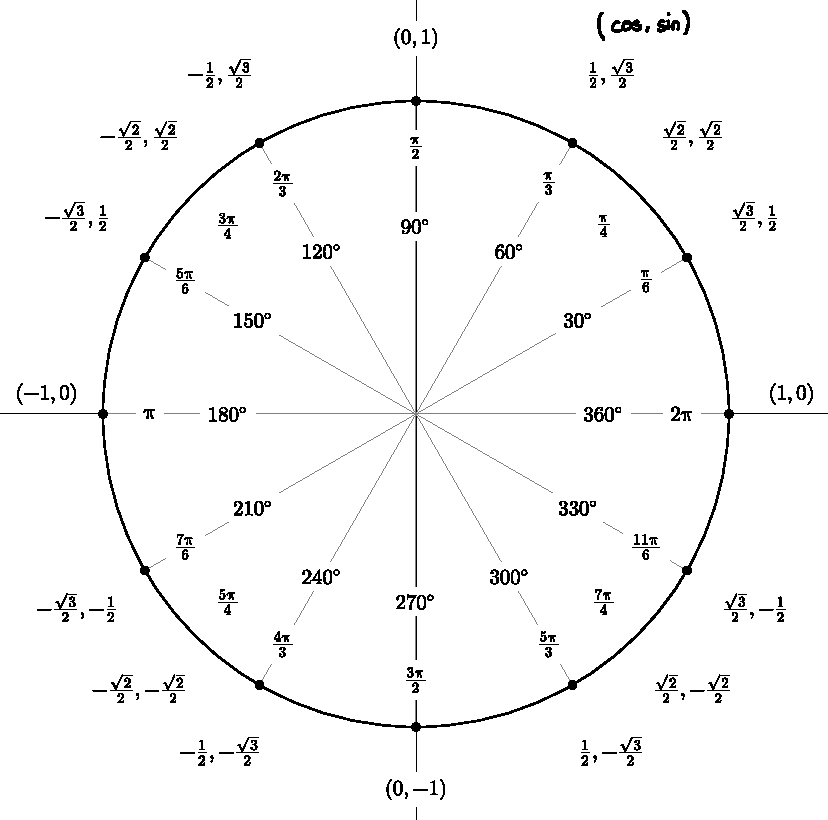
\includegraphics[scale=0.5]{build/pictures/degrees_circle.pdf} 


\begin{flushleft}

\textbf{Periodizität}
\begin{itemize}[leftmargin = *]
\item $\sin (x) & =\sin (x+2 \pi) \qquad \csc (x) = \csc (x+2 \pi)$
\item $\cos (x) & =\cos (x+2 \pi) \qquad \sec (x) = \sec (x+2 \pi)$
\item $\tan (x) & =\tan (x+\pi) \qquad \cot (x) = \cot (x+\pi)$
\item $\sin (x) = -\sin (x+\pi) \qquad \csc (x) = -\csc (x+\pi)$
\item $\cos (x) = -\cos (x+\pi) \qquad \sec (x) = -\sec (x+\pi)$
\end{itemize}

\textbf{Nullstellen}
\begin{itemize}[leftmargin = *]
\item $\sin \phi = 0$: $\phi = k\pi, \, k \in \mathbb{Z}$
\item $\cos \phi = 0$: $\phi = \frac{\pi}{2} + k\pi, \, k \in \mathbb{Z}$
\item $\tan \phi= 0$: $\phi = k\pi, \, k \in \mathbb{Z}$
\end{itemize}


\textbf{Parität}
\begin{itemize}[leftmargin = *]
 \item $\sin(-\alpha) = - \sin(\alpha) \quad \cos(-\alpha) = \cos(\alpha)$
 \item $\tan(-\alpha) = - \tan(\alpha) \quad \cot(-\alpha) = - \cot(\alpha)$
\end{itemize}

\textbf{Ergänzung}
\begin{itemize}[leftmargin = *]
 \item $\sin(\pi - \alpha) = \sin(\alpha) \quad \cos(\pi - \alpha) = - \cos(\alpha)$
 \item $\tan(\pi - \alpha) = -\tan(\alpha) \quad \cot(\pi - \alpha) = - \cot(\alpha)$
\end{itemize}


\textbf{Komplemente}
\begin{itemize}[leftmargin = *]
 \item $\sin(\pi/2 - \alpha) = \cos(\alpha) \quad \cos(\pi/2 - \alpha) = \sin(\alpha)$
 \item $\tan(\pi/2 - \alpha) = -\tan(\alpha) \quad \cot(\pi/2 - \alpha) = -\cot(\alpha)$
\end{itemize}

\textbf{Doppelwinkel}
\begin{itemize}[leftmargin = *]
 \item $\sin(2\alpha) = 2 \sin(\alpha) \cos(\alpha)$
 \item $\cos(2\alpha) = \cos^2(\alpha) - \sin^2(\alpha) = 1 - 2 \sin^2(\alpha)$
 \item $\tan(2\alpha) = \frac{2\tan(\alpha)}{1 - \tan^2(\alpha)}$
\end{itemize}

\textbf{Addition}
\begin{itemize}[leftmargin = *]
 \item $\sin(\alpha + \beta) = \sin(\alpha) \cos(\beta) + \cos(\alpha) \sin(\beta)$
 \item $\cos(\alpha + \beta) = \cos(\alpha) \cos(\beta) - \sin(\alpha) \sin(\beta)$
 \item $\tan(\alpha + \beta) = \frac{\tan(\alpha) + \tan(\beta)}{1 - \tan(\alpha) \tan(\beta)}$
\end{itemize}

\textbf{Subtraktion}
\begin{itemize}[leftmargin = *]
 \item $\sin(\alpha - \beta) = \sin(\alpha) \cos(\beta) - \cos(\alpha)\sin(\beta)$
 \item $\cos(\alpha - \beta) = \cos(\alpha) \cos(\beta) + \sin(\alpha)\sin(\beta)$
 \item $\tan(\alpha - \beta) = \frac{\tan(\alpha) - \tan(\beta)}{1+\tan(\alpha) \tan(\beta)}$
\end{itemize}

\textbf{Multiplikation}
\begin{itemize}[leftmargin = *]
 \item $\sin(\alpha) \sin(\beta) = -\frac{\cos(\alpha + \beta) - \cos(\alpha - \beta)}{2}$
 \item $\cos(\alpha) \cos(\beta) =  \frac{\cos(\alpha + \beta) + \cos(\alpha - \beta)}{2}$
 \item $\sin(\alpha) \cos(\beta) =  \frac{\sin(\alpha + \beta) + \sin(\alpha - \beta)}{2}$
\end{itemize}

\textbf{Potenzen}
\begin{itemize}[leftmargin = *]
 \item $\sin^2(\alpha) = \frac{1}{2}(1-\cos(2\alpha))$
 \item $\cos^2(\alpha) = \frac{1}{2}(1+\cos(2\alpha))$
 \item $\tan^2(\alpha) = \frac{1-\cos(2\alpha)}{1+\cos(2\alpha)}$
\end{itemize}

\textbf{Reduktion}
\begin{itemize}[leftmargin = *]
\item $\sin^2(u) = \frac{1-\cos(2u)}{2}$
\item $\cos^2(u) = \frac{1+\cos(2u)}{2}$
\item $\tan^2(u) = \frac{1-\cos(2u)}{1+\cos(2u)}$

\item $\cos^3(u) = \frac{3 \cos(u)+\cos(3u)}{4}$
\item $\sin^3(u) = \frac{3 \sin(u)-\sin(3u)}{4}$
\item $\tan^3(u) = \frac{3 \sin(u)-\sin(3u)}{3 \cos(u)+\cos(3u)}$ 

\item $\cos^4(u) = \frac{3+ 4 \cos(2u) + \cos(4u)}{8}$
\item $\sin^4(u) = \frac{3- 4 \cos(2u) + \cos(4u)}{8}$
\item $\tan^4(u) = \frac{3+ 4 \cos(2u) + \cos(4u)}{3-4 \cos(2u) + \cos(4u)}$
 
\item $\cos^5(u) = \frac{10 \sin(u) + 5 \sin(3u)+ \sin(5u)}{16}$
\item $\sin^5(u) = \frac{10 \sin(u) - 5 \sin(3u)+ \sin(5u)}{16}$
\item $\tan^5(u) = \frac{10 \sin(u) + 5 \sin(3u)+ \sin(5u)}{10 \sin(u) - 5 \sin(3u)+ \sin(5u)}$ 
\end{itemize}

\textbf{Approximationen ($\rightarrow$ TP)}
\begin{itemize}[leftmargin = *]
\item $\sin (x) \approx x$ für $x \approx 0$
\item $\cos (x) \approx 1-\frac{x^2}{2}$ für $x \approx 0$
\item  $\tan (x) \approx x$ für $x \approx 0$ 
\end{itemize}


\textbf{Diverse}

\begin{itemize}[leftmargin = *]
 \item $\sin^2(\alpha) + \cos^2(\alpha) = 1$
 \item $\cosh^2(\alpha) - \sinh^2(\alpha) = 1$
 \item $\sin(z) = \frac{e^{iz} - e^{-iz}}{2i}$ und $\cos(z) = \frac{e^{iz} + e^{-iz}}{2}$
 \item $\exp (iz) = \cos(z) + i \sin(z)$
 \item $\tan(z)=\frac{\sin(z)}{\cos(z)}\quad \cot(z)=\frac{\cos(z)}{\sin(z)}$
 \item $\sin(x)\leq x$
\end{itemize}

\textbf{Integrale} \\
Sei $\int_{0}^{2\pi} \cos^{a}(t)\sin^{b}(t)dt$
Dann ist:

% Please add the following required packages to your document preamble: %
 \begin{table}[H] \centering \resizebox{\columnwidth}{!}{% 
 \begin{tabular}{llllllll} $a_{\cos}\mid b_{\sin}$ & $0$ & $1$ & $2$ & $3$ & $4$ & $5$ & $6$ \\ $0$ & $2 \pi$ & $0$ & $\pi$ & $0$ & $\frac{3}{4} \pi$ & $0$ & $\frac{5}{8} \pi$ \\ $1$ & $0$ & $0$ & $0$ & $0$ & $0$ & $0$ & $0$ \\ $2$ & $\pi$ & $0$ & $\frac{1}{4} \pi$ & $0$ & $\frac{1}{8} \pi$ & $0$ & $\frac{5}{64} \pi$ \\ $3$ & $0$ & $0$ & $0$ & $0$ & $0$ & $0$ & $0$ \\ $4$ & $\frac{3}{4} \pi$ & $0$ & $\frac{1}{8} \pi$& $0$ & $\frac{3}{64} \pi$ & $0$ & $\frac{3}{128} \pi$ \\ $5$ & $0$ & $0$ & $0$ & $0$ & $0$ & $0$ & $0$ \\ $6$ & $\frac{5}{8} \pi$ & $0$ & $\frac{5}{64} \pi$ & $0$ & $\frac{3}{128} \pi$ & $0$ & $\frac{5}{512} \pi$ \end{tabular}%
 } \end{table}
Falls $a$ oder $b$ ungerade: $0$\\Generell: 	





\textbf{Werte}
\begin{center} 

 \begin{tabular}{c|cccccc}
  deg& $0 \degree $ & $30 \degree $ & $45 \degree $ & $60 \degree $ & $90 \degree $  & $180 \degree $\\
  \hline
  rad & 0 & $\frac{\pi}{6}$ & $\frac{\pi}{4}$ & $\frac{\pi}{3}$ & $\frac{\pi}{2}$ & $\pi$ \\
  cos & 1 & $\frac{\sqrt{3}}{2}$ & $\frac{\sqrt{2}}{2}$ & $\frac{1}{2}$ & 0  & $-1$\\
  sin & 0 & $\frac{1}{2}$ & $\frac{\sqrt{2}}{2}$ & $\frac{\sqrt{3}}{2}$ & 1 & - \\
  tan & 0 & $\frac{1}{\sqrt{3}}$ & 1 & $\sqrt{3}$ & $+\infty$ &-  \\
 \end{tabular}
\end{center} 
 
 
 
 
 \subsection{Grenzwerte}

\begin{center}
  \begin{tabularx}{\linewidth}{XX}
    \toprule
    \textbf{Trigonometrische} & \textbf{Exponential/Log} \\
    \midrule
    $\lim_{x \to 0} \frac{\sin x}{x} = 1$ & $\lim_{x \to 0} \frac{e^x - 1}{x} = 1$ \\
    $\lim_{x \to 0} \frac{\tan x}{x} = 1$ & $\lim_{x \to \infty} \frac{e^x}{x^2} = \infty$ \\
    $\lim_{x \to 0} \frac{1 - \cos x}{x^2} = \frac{1}{2}$ & $\lim_{x \to 0} \frac{e^x - 1}{x^2} = 0$ \\
    $\lim_{x \to 0} \frac{1 - \cos(kx)}{x^2} = \frac{k^2}{2}$ & $\lim_{x \to \infty} \frac{x^3}{e^x} = 0$ \\
    $\lim_{x \to 0^+} \frac{\sin x}{x} = 1$ & $\lim_{x \to 0} \frac{e^{ax} - 1}{x} = a$ \\
    $\lim_{x \to 0^+} \frac{\cos x - 1}{x} = 0$ & $\lim_{x \to 0} \frac{1}{1 + x^2} = 1$ \\
    $\lim_{x \to 0} \frac{\ln(x+1)}{x} = 1$ & $\lim_{x \to \infty} \frac{1}{x} = 0$ \\
    $\lim_{x \to 0} \frac{2x}{2^x} = 0$ & $\lim_{x \to 0^+} \frac{\ln(1+x)}{x} = 1$ \\
    $\lim_{x \to 0} \frac{1 - \cos x}{x^2} = \frac{1}{2}$ & $\lim_{x \to 0^+} \frac{\ln(x)}{x} = -\infty$ \\
    $\lim_{x \to 0^+} \frac{\ln(1 - x)}{x} = -1$ & $\lim_{x \to \infty} \frac{\ln(x)}{x} = 0$ \\
    \midrule
    \textbf{Limits bei Unendlich} & \textbf{Gemischt} \\
    \midrule
    $\lim_{x \to \infty} \frac{x}{1+x^2} = 0$ & $\lim_{x \to 0} \frac{\sqrt{x}}{x} = 0$ \\
    $\lim_{x \to \infty} \frac{\ln(x)}{x} = 0$ & $\lim_{x \to \infty} \frac{x^2 \sin(1/x)}{x} = 0$ \\
    $\lim_{x \to \infty} \frac{x}{\ln x} = \infty$ & $\lim_{x \to 0} \frac{x^2 \sin(1/x)}{x} = 0$ \\
    $\lim_{x \to \infty} \left( 1 + \frac{1}{x} \right)^x = e$ & $\lim_{x \to 0} \frac{2x}{2^x} = 0$ \\
    $\lim_{x \to \infty} \left( 1 + \frac{k}{x} \right)^x = e^{k}$ & $\lim_{x \to 0^+} \frac{\ln(1 - x)}{x} = -1$ \\
    $\lim_{x \to \infty} \frac{n^x}{x!} = 0$ & $\lim_{x \to 0} \frac{e^x - 1}{x^2} = 0$ \\
    $\lim_{x \to 0} \frac{\ln(x+1)}{x} = 1$ & $\lim_{x \to 0} \frac{\ln(x)}{x} = -\infty$ \\
    $\lim_{x \to \infty} \frac{x}{\ln x} = \infty$ & $\lim_{x \to 0^+} \frac{e^x - 1}{x} = 1$ \\
    $\lim_{x \to \infty} \left( 1 + \frac{1}{x} \right)^x = e$ & $\lim_{x \to \infty} \frac{x}{x^2 + 1} = 0$ \\
    \bottomrule
  \end{tabularx}
\end{center}


\subsection{Reihen}
\begin{center}
  \begin{tabularx}{\linewidth}{XX}
    \toprule
    $\sum_{i=1}^{n} i = \frac{n(n+1)}{2}$ & $\sum_{i=1}^{n} i^2 = \frac{n(n+1)(2n+1)}{6}$ \\
    $\sum_{i=1}^{n} i^3 = \frac{n^2 (n+1)^2}{4} $ & $\sum_{i=1}^{\infty} \frac{1}{i^2} = \frac{\pi ^2}{6}$ \\
    $\sum_{i=1}^{ \infty} \frac{1}{i (i+1	)} =1$ &$\sum_{i=0}^{\infty} x^i = \frac{1}{1-x}$\\
     $\sum_{n=0}^{\infty}\frac{(-1)^n}{2n+1} = \frac{\pi}{4}$& $\sum_{n=1}^{\infty}\frac{(-1)^{n+1}}{n} = \ln(2)$  \\
    
    
    \bottomrule
  \end{tabularx}
\end{center}




\subsection{Ableitungen}
\begin{center}
  % the c>{\centering\arraybackslash}X is a workaround to have a column fill up all space and still be centered
  \begin{tabularx}{\linewidth}{c>{\centering\arraybackslash}Xc}
  \toprule
  $\mathbf{F(x)}$ & $\mathbf{f(x)}$ & $\mathbf{f'(x)}$ \\
  \midrule
  $\frac{x^{-a+1}}{-a+1}$ & $\frac{1}{x^a}$ & $-\frac{a}{x^{a+1}}$ \\
  $\frac{x^{a+1}}{a+1}$ & $x^a \ (a \ne -1)$ & $a \cdot x^{a-1}$ \\
  $\frac{1}{k \ln(a)}a^{kx}$ & $a^{kx}$ & $ka^{kx} \ln(a)$ \\
  $\ln |x|$ & $\frac{1}{x}$ & $-\frac{1}{x^2}$ \\
  $\frac{2}{3}x^{3/2}$ & $\sqrt{x}$ & $\frac{1}{2\sqrt{x}}$\\
  $\frac{n}{n+1}x^{\frac{1}{n}+1}$ & $\sqrt[n]{x}$ & $\frac{1}{n}x^{\frac{1}{n}-1}$\\
  $-\cos(x)$ & $\sin(x)$ & $\cos(x)$ \\
  $\sin(x)$ & $\cos(x)$ & $-\sin(x)$ \\
  $\frac{1}{2}(x-\frac{1}{2}\sin(2x))$ & $\sin^2(x)$ & $2 \sin(x)\cos(x)$ \\
  $\frac{1}{2}(x + \frac{1}{2}\sin(2x))$ & $\cos^2(x)$ & $-2\sin(x)\cos(x)$ \\
  \multirow{2}*{$-\ln|\cos(x)|$} & \multirow{2}*{$\tan(x) = \frac{\sin}{\cos}$} & $\frac{1}{\cos^2(x)}$  \\
  & & $1 + \tan^2(x)$ \\
  $\cosh(x)$ & $\sinh(x)$ & $\cosh(x)$ \\
  $\log(\cosh(x))$ & $\tanh(x)$ & $\frac{1}{\cosh^2(x)}$ \\
  $\ln (\sin(x))$ & $\cot(x)$ & $-\frac{1}{\sin^2(x)}$ \\
  $\frac{1}{c} \cdot e^{cx}$ & $e^{cx}$ & $c \cdot e^{cx}$ \\
  $x(\ln |x| - 1)$ & $\ln |x|$ & $\frac{1}{x}$ \\
  $\frac{1}{2}(\ln(x))^2$ & $\frac{\ln(x)}{x}$ & $\frac{1 - \ln(x)}{x^2}$ \\
  $\frac{x}{\ln(a)} (\ln|x| -1)$ & $\log_a |x|$ & $\frac{1}{\ln(a)x}$ \\
  
 $\frac{1}{2} \log \left(x^2+1\right)$  & $\frac{x}{1+x^2}$ & $\frac{1-x^2}{\left(1+x^2\right)^2}$
  \\
- &$c\cdot \arcsin(\frac{x}{c})$& $\frac{1}{\sqrt{1-\frac{x^2}{c^2}}}$ \\
- &$c\cdot \arccos(\frac{x}{c})$& $\frac{-1}{\sqrt{1-\frac{x^2}{c^2}}}$ \\
- &$\frac{b\cdot \arctan(\frac{x}{ab})}{a}$& $\frac{1}{a^2+\frac{x^2}{b^2}}$ \\
- &$\operatorname{arcsinh}(x)$& $\frac{1}{\sqrt{x^2 +1}}$ \\
- &$\operatorname{arccosh}(x)$& $\frac{1}{\sqrt{x-1}\sqrt{x+1}}$ \\
- &$\frac{b\cdot \operatorname{arctanh}(\frac{x}{ab})}{a}$& $\frac{1}{a^2-\frac{x^2}{b^2}}$ \\

  \bottomrule
  \end{tabularx}
\end{center}









\subsection{Indefinite Integrale}
\begin{center}
 \begin{tabularx}{\linewidth}{>{\centering\arraybackslash}X>{\centering\arraybackslash}X}
  \toprule
  $\mathbf{f(x)}$ & $\mathbf{F(x)}$ \\
  \midrule
  $\int f'(x) f(x) \dx$ & $\frac{1}{2}(f(x))^2$ \\
  $\int \frac{f'(x)}{f(x)} \dx$ & $\ln|f(x)|$ \\
  $\int_{-\infty}^\infty e^{-x^2} \dx$ & $\sqrt{\pi}$ \\
  $\int (ax+b)^n \dx$ & $\frac{1}{a(n+1)}(ax+b)^{n+1}$ \\
  $\int x(ax+b)^n \dx$ & $\frac{(ax+b)^{n+2}}{(n+2)a^2} - \frac{b(ax+b)^{n+1}}{(n+1)a^2}$ \\
  $\int (ax^p+b)^n x^{p-1} \dx$ & $\frac{(ax^p+b)^{n+1}}{ap(n+1)}$ \\
  $\int (ax^p + b)^{-1} x^{p-1} \dx$ & $\frac{1}{ap} \ln |ax^p + b|$ \\
  $\int \frac{ax+b}{cx+d} \dx$ & $\frac{ax}{c} - \frac{ad-bc}{c^2} \ln |cx +d|$ \\
  $\int \frac{1}{x^2+a^2} \dx$ & $\frac{1}{a} \arctan \frac{x}{a}$ \\
  $\int \frac{1}{x^2 - a^2} \dx$ & $\frac{1}{2a} \ln\left| \frac{x-a}{x+a} \right|$ \\
  $\int \sqrt{a^2+x^2} \dx $ & $\frac{x}{2}f(x) + \frac{a^2}{2}\ln(x+f(x))$ \\

   
%here   
   
   
  $\int \frac{1}{(x+a)^2}dx$& $-\frac{1}{a+x}$ \\
$\int \frac{1}{(x+a)^3}dx$& $-\frac{1}{2(a+x)^2}$ \\
$\int \frac{1}{(x+a)^t}dx$& $\frac{1}{(1-t)(x+a)^{t+1}}$ \\
$\int \frac{x}{(x+a)^2}dx$& $\frac{a}{a+x}+\log |a+x|$ \\
$\int \frac{x}{(x+a)^3}dx$& $-\frac{a+2x}{2(a+x)^2}$ \\
$\int \frac{1}{ax^2+bx+c}dx$& $\frac{2 \arctan\left(\frac{2ax+b}{\sqrt{4ac-b^2}} \right)}{\sqrt{4ac-b^2}}$\\

  $\int \sin(kx)\cdot \cos(kx)dx$ & $-\frac{1}{4k}\cos(2kx)=\frac{-(\cos(x))^2}{2}$\\
  


 $\int \cos^n(x) d x$ & $\frac{n-1}{n} \int \cos^{n-2}(x) d x+\frac{\cos^{n-1}(x) \sin (x)}{n}$ \\
$ \int \sin^n(x) d x $ & $\frac{n-1}{n} \int \sin ^{n-2}(x) d x-\frac{\cos (x) \sin ^{n-1}(x)}{n}$\\


$\int \sin \cos dx$ & $\frac{-1}{2}\cos^2$\\
  $\int \frac{\cos}{ \sin} dx$ & $\log(\cos(x))$\\
  
  \bottomrule
 \end{tabularx}
\end{center}




\subsection{Multiple Choice}


\scriptsize

%Sets
\textbf{Welche der folgenden Teilmengen von $\mathbb{R}^2$ ist kompakt?}

\begin{itemize}[leftmargin = *]
\item[\textcolor{green}{W}] $B=\left\{(a, b, c) \in \mathbb{R}^3 \mid a, b, c \in \mathbb{Z}\right.$ und $\left.a^2+b^2+c^2<2024\right\}$\textcolor{Emerald}{endlich viele Punkte $\Rightarrow$ Kompakt}
\item[\textcolor{green}{W}] $F=\left\{(x, f(x)) \in \mathbb{R}^{n+1}\left|x \in \mathbb{R}^n,|x| \leq 1\right\}\right.$, wobei $f: \mathbb{R}^n \rightarrow \mathbb{R}$ eine stetige Funktion ist. \textcolor{Emerald}{S.3.2.15 $\Rightarrow F $ beschränkt. Kompakt: Sei $F \ni\left(x_k, y_k\right) \rightarrow$ $(x, y)$. Dann ist $y_k=f\left(x_k\right)$ und aus der Stetigkeit von $f$ und $x_k \rightarrow x$ folgt, dass $y=f(x)$, also $(x, y) \in F$. Somit ist $F$ kompakt.}
\item[\textcolor{green}{W}] $\left\{(x, y) \in \mathbb{R}^2 \mid 4 x^4+2024 y^{2024} \leq 1\right\}$  

\item[\textcolor{green}{W}]  $\left\{(x, y) \in \mathbb{R}^2 \mid x \in[-1,1], y \in\left[-e^x, e^x\right]\right\}$

\item[\textcolor{green}{W}] $C=\left\{(\sin (1 / \theta) \cos \theta, \sin (1 / \theta) \sin \theta, \theta) \in \mathbb{R}^3 \mid 0<\theta \leq 1\right\} \cup\left\{(x, y, 0) \in \mathbb{R}^3 \mid x^2+y^2 \leq 1\right\}$

\item[\textcolor{red}{F}]  $\left\{(x, y) \in \mathbb{R}^2 \mid x^2-y^2 \leq 1\right\}$ \textcolor{Emerald}{nicht beschränkt}
\item[\textcolor{red}{F}]  $\left\{(x, y) \in \mathbb{R}^2 \mid x^3+y^3 \leq 1\right\}$ \textcolor{Emerald}{nicht beschränkt}
\item[\textcolor{red}{F}]  $\left\{\left(\sqrt{1-t^2}, \sqrt{1+t^2}\right) \mid t \in(-1,1)\right\}$ \textcolor{Emerald}{nicht abgeschlossen}
\item[\textcolor{red}{F}]  $\left\{(x, y) \in \mathbb{R}^2 \mid y \geq 0\right\}$. \textcolor{Emerald}{nicht beschränkt}
\item[\textcolor{red}{F}]  $\{(t, \arctan (t)) \mid t \in \mathbb{R}\}$ \textcolor{Emerald}{nicht beschränkt}
\item[\textcolor{red}{F}]  $\left\{(x, y) \in \mathbb{R}^2 \mid x^2+y^2<1\right\}$ \textcolor{Emerald}{nicht abgeschlossen}


\end{itemize}



\textbf{Bestimmen Sie ob die folgenden Aussagen richtig oder falsch}

\begin{itemize}[leftmargin = *]
\item [\textcolor{green}{W}] $g(x)=x \cdot|x|$ ist $C^1(\mathbb{R}, \mathbb{R})$. \textcolor{Emerald}{Mit Fallunterscheidung $g^{\prime}(x)=2 |x|$, $g$ in $C^1$ aber nicht $C^2$}
\item[\textcolor{green}{W}] Falls $A \subseteq \mathbb{R}^n$ abgeschlossen ist, dann ist $A^c=\mathbb{R}^n \backslash A$ offen \textcolor{Emerald}{Beweis per Widerspruch}
\item[\textcolor{green}{W}] Sei $f:[0,1]^n \rightarrow \mathbb{R}$ stetig. Dann ist $f$ beschränkt. \textcolor{Emerald}{TRM 3.2.15}
\item[\textcolor{green}{W}] Eine Funktion $h: \mathbb{R}^n \rightarrow \mathbb{R}^m$ ist genau dann stetig differenzierbar, wenn alle Richtungsableitungen existieren und stetig sind.
\item[\textcolor{red}{F}] Sei pr: $\mathbb{R}^2 \rightarrow \mathbb{R},(x, y) \mapsto x$ und $A \subseteq \mathbb{R}^2$ abgeschlossen. Dann ist auch $\operatorname{pr}(A) \subseteq \mathbb{R}$ abgeschlossen. \textcolor{Emerald}{GgBsp: $A=\left\{(x, y) \in \mathbb{R}^2 \mid e^{-|y|} \leq x \leq 2 e^{-|y|}\right\}$. Dann ist $\operatorname{pr}(A)=(0,2]$}

\item[\textcolor{red}{F}] Die Menge $O \subseteq \mathbb{R}^n$ ist genau dann offen, wenn $O$ nicht abgeschlossen ist. \textcolor{Emerald}{GgBsp: $n=1$ und $O=(0,1]$. Dann ist $O$ weder abgeschlossen noch offen.}
\item[\textcolor{red}{F}]  Sei $f:[-1,1]^n \backslash\{0\} \rightarrow \mathbb{R}$ stetig. Dann ist $f$ beschränkt.  \textcolor{Emerald}{GgBsp: $f:[-1,1]^n \backslash$ $\{0\} \rightarrow \mathbb{R}, x \mapsto\|x\|^{-1}$}
\item[\textcolor{red}{F}] Ist $A \subset \mathbb{R}^n$ abgeschlossen, dann ist auch $f(A)$ abgeschlossen für stetige $f$\textcolor{Emerald}{GgBsp:$f(x)=\arctan(x)$}

\item[\textcolor{red}{F}] Ist $D \subset \mathbb{R}^m$ beschränkt, dann ist auch $f^{-1}(D)$ beschränkt.\textcolor{Emerald}{GgBsp:$f(x)=2$}
\end{itemize}

 \textcolor{Emerald}{}

\textbf{Die Menge $U=\left\{(x, y) \in \mathbb{R}^2 \mid x \neq y\right.$ oder $\left.x<0\right\} \subset \mathbb{R}^2$ ist: }

\begin{itemize}[leftmargin = *]
\item[\textcolor{green}{W}] Sternförmig, aber nicht konvex
\end{itemize}


% Stetigkeit/diffbar


\textbf{Seien $n \geq 1, m \geq 2$ und $f: \mathbb{R}^n \rightarrow \mathbb{R}^m$ eine Funktion
$f(x)=\left(f_1(x), f_2(x), \ldots, f_m(x)\right)$
wobei $f_1, f_2, \ldots, f_m: \mathbb{R}^n \rightarrow \mathbb{R}$. Welche der folgenden Aussagen sind richtig?}

\begin{itemize}[leftmargin = *]
\item[\textcolor{green}{W}] Wenn es $1 \leq i \leq m$ gibt, sodass $f_i$ injektiv ist, dann ist $f$ auch injektiv.
\item[\textcolor{green}{W}] Wenn $f$ stetig ist, dann ist $f_i$ stetig für alle $1 \leq i \leq m$.	
\item[\textcolor{green}{W}] Wenn $f$ surjektiv ist, dann gilt auch für jedes $1 \leq i \leq m$. dass $f_i$ surjektiv ist.
\item[\textcolor{green}{W}] Wenn $f_i$ stetig sind für alle $1 \leq i \leq m$, dann ist $f$ auch stetig.
\item[\textcolor{red}{F}]  Wenn $f$ injektiv ist, dann gilt auch für jedes $1 \leq i \leq m$, dass $f_i$ injektiv ist.\textcolor{Emerald}{GgBsp: $f=(x,1)$}

\item[\textcolor{red}{F}] Gibt es $1 \leq i \leq m$, sodass $f_i$ surjektiv ist, dann ist $f$ auch surjektiv. \textcolor{Emerald}{GgBsp: $f=(x,1)$}
  
\end{itemize}







\textbf{Welche Funktion ist Differenzierbar:}

\begin{itemize}[leftmargin = *]
\item[\textcolor{green}{W}] $f: \mathbb{R}^2 \rightarrow \mathbb{R}, f(x, y)=x^2+e^{2 y}$
\item[\textcolor{red}{F}]  $f: \mathbb{R}^2 \rightarrow \mathbb{R}, f(x, y)=|x|+|y|$ \textcolor{Emerald}{Da $|x|$ nicht diffbar ist.}
\item[\textcolor{red}{F}] $f: \mathbb{R}^2 \rightarrow \mathbb{R}, f(x, y)= \begin{cases}\frac{x^2 y}{x^4+y^4} & \text { if }(x, y) \neq(0,0) \\ 0 & \text { if }(x, y)=(0,0)\end{cases}$ \textcolor{Emerald}{}
\item[\textcolor{red}{F}] $f: \mathbb{R}^2 \rightarrow \mathbb{R}, f(x, y)= \begin{cases}\frac{(x+y) y}{x^2+y^2} & \text { if }(x, y) \neq(0,0) \\ 0 & \text { if }(x, y)=(0,0)\end{cases}$  \textcolor{Emerald}{Nicht stetig $\Rightarrow$ nicht diffbar}
\end{itemize}


\textbf{Sei $f: \mathbb{R}^2 \rightarrow \mathbb{R}$. Welche partiellen Ableitungen von $f$ garantieren, dass $f$ differenzierbar ist? }

\begin{itemize}[leftmargin = *]
\item[\textcolor{green}{W}] $f_x(x, y)=|x|, f_y(x, y)=0$ \textcolor{Emerald}{Beide existieren und sind stetig}
\item[\textcolor{red}{F}]  $f_x(x, y)=\ln (x), f_y(x, y)=x$
\textcolor{Emerald}{$\ln(x)$ nicht definiert für $x<0$}
\item[\textcolor{red}{F}]   $f_x(x, y)=0, f_y(x, y)=\frac{1}{x}$ \textcolor{Emerald}{$\frac{1}{x}$ nicht stetig bei $0$}
\item[\textcolor{red}{F}]  $f_x(x, y)=\left\{\begin{array}{ll}0 & x<0 \\ 1 & x \geq 0\end{array}, f_y(x, y)=5\right.$ \textcolor{Emerald}{$f_x$ nicht stetig bei $0$}
\end{itemize}











\textbf{ Sei $f$ eine Funktion $\mathbb{R}^n \rightarrow \mathbb{R}^m$. Welche der folgenden Bedingungen ist äquivalent \textcolor{Emerald}{$=\Leftrightarrow$ (falls hinreichend $=\Rightarrow$)}  dazu, dass $f$ differenzierbar ist?}

\begin{itemize}[leftmargin = *]
\item[\textcolor{green}{W}] Für jedes $x_0 \in \mathbb{R}^n$ gibt es eine $m \times n$ Matrix $A$, sodass $f(x)=f\left(x_0\right)+A \cdot\left(x-x_0\right)+o\left(\left\|x-x_0\right\|\right)$.\textcolor{Emerald}{$\Leftrightarrow$ f diffbar}    
\item[\textcolor{red}{F}]  $f$ ist stetig. \textcolor{Emerald}{$\Leftarrow$ f diffbar} 
\item[\textcolor{red}{F}]  Alle Richtungsableitungen von $f$ existieren. \textcolor{Emerald}{$\Leftarrow$ f diffbar} 
\item[\textcolor{red}{F}]  Alle partiellen Ableitungen von $f$ existieren und sind stetig. \textcolor{Emerald}{$\Rightarrow$ f diffbar} 
\end{itemize}


\begin{itemize}[leftmargin = *]
\item[\textcolor{green}{W}] Wenn $f$ in $(0,0)$ differenzierbar ist, dann ist $f$ auch stetig bei $(0,0)$. \textcolor{Emerald}{Prop. 3.4.4}
\item[\textcolor{red}{F}]  Wenn $f$ stetig bei $(0,0)$ ist, dann gibt es $u \in \mathbb{R}^n$, sodass $D_u f(0,0)$ existiert. \textcolor{Emerald}{GgBsp: $f(x)=\|x\|$ ist stetig, aber hat keine Richtungsableitung in 0.}
\item[\textcolor{red}{F}] Wenn alle Richtungsableitungen von $f$ in $(0,0)$ existieren, dann ist $f$ auch stetig bei $(0,0)$.  \textcolor{Emerald}{GgBsp: $f(x, y)=\frac{x y}{x^2+y^2}$}
\item[\textcolor{red}{F}]  Wenn beide partielle Ableitungen von $f$ in $(0,0)$ existieren, dann ist $f$ auch stetig bei $(0,0)$. \textcolor{Emerald}{GgBsp: $f(x, y)=\frac{x y}{x^2+y^2}$}
\end{itemize}


\textbf{Wir identifizieren den Raum $M(2, \mathbb{R})$ der $2 \times 2$ Matrizen mit reellen Koeffizienten mit $\mathbb{R}^4$ via der Abbildung$
\begin{smallmatrix}
a & b \\
c & d
\end{smallmatrix} \mapsto\left(a,b,c,d\right)^{T}$ Sei $M \in M(2, \mathbb{R})$ fest. Welche der folgenden Sätze sind richtig? }

\begin{itemize}[leftmargin = *]
\item[\textcolor{green}{W}] Die Funktion det: $A \mapsto \operatorname{det} A$ ist differenzierbar auf $M(2, \mathbb{R})$.
\item[\textcolor{green}{W}] Die Funktion $\Pi_M: A \mapsto M \cdot A$ ist auf $M(2, \mathbb{R})$ differenzierbar.
\item[\textcolor{red}{F}]  Die Funktion $\operatorname{tr}: A \mapsto \operatorname{tr} A$ ist nicht auf ganz $M(2, \mathbb{R})$ differenzierbar. 
\textcolor{Emerald}{Für alle gilt: Darstellbar als polynom und somit $C^{\infty}$}
\end{itemize}



\textcolor{Emerald}{nicht abgeschlossen}


\textbf{Wenn für eine Funktion $f: \mathbb{R}^3 \rightarrow \mathbb{R}$ alle Richtungsableitungen existieren, dann ist $f$ differenzierbar.}

\begin{itemize}[leftmargin = *]
\item[\textcolor{green}{W}] Falsch
\item[\textcolor{red}{F}]  Wahr \textcolor{Emerald}{GgBsp $g(x, y) =x^2 y /\left(x^2+y^2\right)$ für $(x, y) \neq$ $(0,0)$ ansonsten $g(0,0)=0$.
}
\end{itemize}

\textbf{Seien $f: \mathbb{R}^n \rightarrow \mathbb{R}$ und $g: \mathbb{R}^n \rightarrow \mathbb{R}^n$ zweimal stetig differenzierbare Funktionen, $n \geq 2$. Welche Aussagen gelten?}

\begin{itemize}[leftmargin = *]
\item[\textcolor{green}{W}] $J_g(x)$ ist eine $n \times n$-Matrix.
\item[\textcolor{green}{W}] $H_f(x)$ ist symmetrisch.\textcolor{Emerald}}{Def. 3.5.1 mit Prop. 3.5.4}
\item[\textcolor{red}{F}]   $J_q(x)$ ist symmetrisch.\textcolor{Emerald}}{GgBsp: $g(x)=\left(x_2, 0, \ldots, 0\right)$.}
\item[\textcolor{red}{F}]  $\nabla f(x)$ ist eine $n \times n$-Matrix. \textcolor{Emerald}}{$\nabla f(x)$ ist ein Vektor}
\end{itemize}



\textbf{Sei $f: \mathbb{R}^n \rightarrow \mathbb{R}, n \geq 1$ eine $C^1$-Funktion und sei $x_0$ ein kritischer Punkt von $f$ (das heisst $\nabla f\left(x_0\right)=0$ ). Was können wir über die Tangentialebene am Graphen von $f$ an der Stelle $x_0$ sagen? }

\begin{itemize}[leftmargin = *]
\item[\textcolor{green}{W}] Sie ist horizontal. \textcolor{Emerald}{$TE(p)=f\left(x_0\right)+0$}
\end{itemize}



\textbf{ Sei $f: \mathbb{R}^3 \rightarrow \mathbb{R},(x, y, z) \mapsto f(x, y, z)$ eine glatte Funktion, so dass$
\nabla f\left(-\frac{\sqrt{2}}{2},-\frac{\sqrt{6}}{2},-\sqrt{2}\right)=(-\sqrt{2},-\sqrt{6},-2 \sqrt{2})$ Seien $(r, \theta, \varphi)$ die Kugelkoordinaten (d.h. $x=r \sin \theta \cos \varphi, y=r \sin \theta \sin \varphi$ und $z=r \cos \theta$ ). Der Wert von$\frac{\partial f}{\partial r}\left(2, \frac{5 \pi}{4}, \frac{\pi}{3}\right)$ist:}

\begin{itemize}[leftmargin = *]
\item[\textcolor{green}{W}] $4$
 \textcolor{Emerald}{Kettenregel: $\frac{\partial f}{\partial r}(r, \theta, \varphi) = \nabla g(f(t)) \cdot \frac{\partial f}{\partial r}$}

\end{itemize}






% Umkehrsatz


\textbf{Ist $f: \mathbb{R}^2 \rightarrow \mathbb{R}$ eine stetig differenzierbare Funktion, deren Jacobimatrix überall invertierbar ist, dann ist $f$ injektiv. }

\begin{itemize}[leftmargin = *]
\item[\textcolor{green}{W}] Falsch 
\item[\textcolor{red}{F}] Wahr  \textcolor{Emerald}{S 3.10.2 macht keine globalen Aussagen. Gilt jedoch für $n=1$, da $f'(0)\neq 0$ und $f$ somit strikt wachsend/fallend ist}

\end{itemize}


% Differenzialgeichungen


\textbf{Welche der folgenden ODEs hat nicht-triviale beschränkte Lösungen für $x \rightarrow+\infty$ ?}

\begin{itemize}[leftmargin = *]
\item[\textcolor{green}{W}] $f^{\prime \prime}(x)+3 f^{\prime}(x)+2 f(x)=0$ \textcolor{Emerald}{$f(x)=C_1 e^{-x}+C_2 e^{-2 x}$}
\item[\textcolor{red}{F}]  $f^{\prime \prime}(x)-5 f^{\prime}(x)+6 f(x)=0$ \textcolor{Emerald}{$f(x)=C_1 e^{2 x}+C_2 e^{3 x}$}
\item[\textcolor{red}{F}]  $f^{\prime \prime}(x)-2 f^{\prime}(x)+f(x)=0$   \textcolor{Emerald}{$f(x)=\left(C_1+C_2 x\right) e^x$}
\end{itemize}




\textbf{Wie viele maximale Lösungen hat das Anfangswertproblem $y^{\prime}=\sqrt[3]{y^2}, y(0)=0$ ?}

\begin{itemize}[leftmargin = *]
\item[\textcolor{green}{W}] Unendlich viele. \textcolor{Emerald}{Für jedes $T\geq 0$ ist die Lösung: $y(x)= \begin{cases}0 & \text { für } x \leq T \\ (x-T)^3 / 27 & \text { für } x>T .\end{cases}$} 
\item[\textcolor{red}{F}] Keine. 
\item[\textcolor{red}{F}] Genau eine.  
\item[\textcolor{red}{F}] Genau zwei.  
\end{itemize}

\textbf{Wie viele Lösungen hat eine lineare ODE, deren Koeffizienten und Inhomogenität stetig sind?}

\begin{itemize}[leftmargin = *]
\item[\textcolor{green}{W}] Unendlich viele. \textcolor{Emerald}{Ordnung $k\geq 1$, S. 2.2.3 $\Rightarrow$ affinen Raum von dim $k$} 
\item[\textcolor{red}{F}] Es hängt von der ODE ab.
\item[\textcolor{red}{F}] Genau eine.    
\end{itemize}







\textbf{Betrachten Sie die gewöhnliche Differentialgleichung $y^{(4)}-y^{\prime}=y$. Welche Dimension hat der Vektorraum der Lösungen mit $y(2)=y^{\prime}(2)=1$ ? }

\begin{itemize}[leftmargin = *]
\item[\textcolor{green}{W}] die Lösungen bilden gar keinen Vektorraum. \textcolor{Emerald}{Es müsste gelten $y(2)=1 \neq 2 = y(2)+y(2)$}
\item[\textcolor{red}{F}] $0$  
\item[\textcolor{red}{F}] $2$  
\item[\textcolor{red}{F}] $3$  
\end{itemize}

\textbf{Betrachten Sie die folgende ODE $y^{(4)}+2 y^{(2)}=0$ Welche der folgenden Sätze sind richtig?}
\textcolor{Emerald}{$y=C_1 e^{i \sqrt{2} t}+C_2 e^{-i \sqrt{2} t}+C_3+C_4 t$}

\begin{itemize}[leftmargin = *]
\item[\textcolor{green}{W}] Der Lösungsraum mit $y(0)=0$ ist ein 3 -dimensionaler Vektorraum. \textcolor{Emerald}{$C_1+C_2+C_3=0$., $3$-dim}
\item[\textcolor{red}{F}]   Der Lösungsraum mit $y(0)=1$ ist ein 3-dimensionaler Vektorraum. \textcolor{Emerald}{ $y_1(0)=y_2(0)$, dann ist $\left(y_1+y_2\right)(0)=y_1(0)+y_2(0)=2$, also ist $y_1+y_2$ keine Lösung des AWP}
\item[\textcolor{red}{F}] Der Lösungsraum mit $\lim _{t \rightarrow+\infty} y(t)=0$ ist ein 2-dimensionaler Vektorraum. \textcolor{Emerald}{$C_1=C_2=C_3=C_4=0$, $0$-dim}
\item[\textcolor{red}{F}] Der Lösungsraum mit $y^{\prime}(0)=0$ ist ein 2-dimensionaler Vektorraum. \textcolor{Emerald}{$i \sqrt{2} C_1-i \sqrt{2} C_2+C_4=0$, $3$-dim}

\end{itemize}




\textbf{Für welches $a \in \mathbb{R}$ hat das Anfangswertproblem $y^{\prime}=-2 x y^2, y(0)=a$ eine auf ganz $\mathbb{R}$ definierte Lösung? }

\begin{itemize}[leftmargin = *]
\item[\textcolor{green}{W}] $a=0$ \textcolor{Emerald}{Triviale Lösung}
\item[\textcolor{green}{W}]   $a=1$ \textcolor{Emerald}{Lösung $y(x)=\frac{1}{x^2+c}$, definiert für $c>0$ da dann $\forall x \cdot x^2 + c \neq 0$}
\item[\textcolor{red}{F}] $a=-1$
\item[\textcolor{red}{F}] $a=-2$

\end{itemize}



% Vektorfelder


\textbf{Sei $f: \mathbb{R}^2 \rightarrow \mathbb{R}^2$ das Vektorfeld $f(x, y)=\left(x^3+2 x y, y^2+x^2\right)$ und $\gamma:[0,1] \rightarrow \mathbb{R}^2$ der Weg $\gamma(t)=\left(\sin (t \pi) e^{t^2}, 3 \sin (t \pi / 2) e^{t^3-t}\right)$. Was ist der Wert des Wegintegrals von $f$ entlang $\gamma$ ? }

\begin{itemize}[leftmargin = *]
\item[\textcolor{green}{W}] $9$
\item[\textcolor{red}{F}]    $0$
\item[\textcolor{red}{F}]   $3$
\item[\textcolor{red}{F}]  $27$
\end{itemize}

\textbf{Das Vektorfeld $f:(0, \infty) \times(0, \infty) \rightarrow \mathbb{R}^2$,$
f(x, y)=(\cos (1 / x) \sin (1 / y), \quad \sin (1 / x) \cos (1 / y))$ ist konservativ.}



\begin{itemize}[leftmargin = *]
\item[\textcolor{green}{W}] Falsch
\item[\textcolor{red}{F}]  Wahr
\end{itemize}

\textbf{Welche der folgenden Aussagen sind wahr?}

\begin{itemize}[leftmargin = *]
\item[\textcolor{green}{W}] Sei $f: \mathbb{R}^2 \rightarrow \mathbb{R}^2, f(x, y)=\left(e^{x+y^2}, 0\right)$ und $\gamma:[-\pi, \pi] \rightarrow \mathbb{R}^2, \gamma(t)=(0, \sin (t))$. Dann $\int_\gamma f(s) \cdot d \vec{s}=0$. \textcolor{Emerald}{$x$ und $y$-Komponente beide $0$}
\item[\textcolor{green}{W}] Seien $\gamma, \sigma:[0,1] \rightarrow \mathbb{R}^2$ Wege mit $\sigma(t)=\gamma\left(t^9\right)$. Dann gilt $\int_\gamma f(s) \cdot d \vec{s}=\int_\sigma f(s) \cdot d \vec{s}$. \textcolor{Emerald}{orientierte Umparametrisierung}
\item[\textcolor{red}{F}]   Haben zwei Wege $\gamma$ und $\sigma$ das gleiche Bild, so gilt $\int_\gamma f(s) \cdot d \vec{s}=\int_\sigma f(s) \cdot d \vec{s}$.

\end{itemize}



% Integrale

\textbf{Sei $D=\left\{(x, y) \in \mathbb{R}^2 \mid x^2+y^2 \geq 1\right\}$. Das uneigentliche Integral$
\int_D \frac{1}{x^4+2 x^2 y^2+y^4} d x d y \ldots$
 }

\begin{itemize}[leftmargin = *]
\item[\textcolor{green}{W}] $\ldots$ ist gleich $\pi$.
\item[\textcolor{red}{F}] ...divergiert.
\item[\textcolor{red}{F}]   $\ldots$ ist gleich $-2 \pi$.
\item[\textcolor{red}{F}] $\ldots$ ist gleich $1 / 2$.
\end{itemize}


\textbf{Welchen Wert hat $\int_0^1 \int_{y^4}^1 y^3 e^{x^2} d x d y ?$
 }

\begin{itemize}[leftmargin = *]
\item[\textcolor{green}{W}] $(e-1) / 8$  \textcolor{Emerald}{Integriere $\int_0^1 \int_0^{\sqrt[4]{x}} y^3 e^{x^2} d y d x$}  
\end{itemize}

\textbf{
Wenn $f: \mathbb{R}^2 \rightarrow \mathbb{R}$ stetig und positiv ist, und der Grenzwert$
\lim _{R \rightarrow \infty} \int_{[-R, R]^2} f(x, y) d x d y$ existiert, dann existiert auch der Grenzwert $
\lim _{R \rightarrow \infty} \int_{B_R(0)} f(x, y) d x d y$ und die beiden Grenzwerte sind gleich.}

\begin{itemize}[leftmargin = *]
\item[\textcolor{green}{W}] Wahr  
\item[\textcolor{red}{F}] Falsch
\end{itemize}

\textbf{Welche der folgenden Aussagen sind wahr?}

\begin{itemize}[leftmargin = *]
\item[\textcolor{green}{W}] Wenn $\lim _{\|x\| \rightarrow \infty} f(x)$ existiert und nicht null ist, dann ist das uneigentliche Integral $\int_{\mathbb{R}^n} f d x$ nicht endlich.\textcolor{Emerald}{Wenn $\lim _{x \rightarrow \infty} f(x)=c>0$, dann gibt es ein $R>0$, so dass $f(x)>c / 2$, wenn $|x|>R$, also $\int_{\mathbb{R}^n} f d x \geq \int_{\mathbb{R}^n \backslash B_R} \frac{c}{2} d x=+\infty$}
\item[\textcolor{red}{F}] Wenn $\lim _{\|x\| \rightarrow \infty} f(x)$ nicht existiert, dann ist das uneigentliche Integral $\int_{\mathbb{R}^n} f d x$ nicht endlich.  
\item[\textcolor{red}{F}]   Wenn das uneigentliche Integral $\int_{\mathbb{R}^n} f d x$ existiert und endlich ist, dann gilt $\lim _{\|x\| \rightarrow \infty} f(x)=0$
\item[\textcolor{red}{F}] Wenn $f: \mathbb{R}^n \rightarrow[0,+\infty)$ eine nicht-negative stetige Funktion mit $\lim _{\|x\| \rightarrow \infty} f(x)=0$ ist, dann existiert das uneigentliche Integral $\int_{\mathbb{R}^n} f d x$ und ist endlich.\textcolor{Emerald}{GgBsp: $f(x)=\frac{1}{1+|x|}$}
\end{itemize}




% Transformationssatz

\textbf{Sei $f: \mathbb{R}^n \rightarrow \mathbb{R}$ eine stetige Funktion und $r>0$. Dann ist das Integral$
\int_{[0, r]^n} f(x) d x$ gleich}

\begin{itemize}[leftmargin = *]
\item[\textcolor{green}{W}] $r^n \int_{[0,1]^n} f(r x) d x$
\item[\textcolor{red}{F}] $r^n \int_{[0,1]^n} f(x / r) d x$
\item[\textcolor{red}{F}] $r^{-n} \int_{[0,1]^n} f(r x) d x$
\item[\textcolor{red}{F}] $r^{-n} \int_{[0,1]^n} f(x / r) d x$
\end{itemize}


\textbf{Sei $f: \mathbb{R}^n \rightarrow \mathbb{R}$ eine stetige Funktion und $B_r(0):=\left\{x \in \mathbb{R}^n\right.$ sodass $\left.\|x\| \leq r\right\}$, wobei $r>0$. Das Integral$
\int_{B_r(0)} f(x) \mathrm{d} x$ kann auch geschrieben werden als }

\begin{itemize}[leftmargin = *]
\item[\textcolor{green}{W}] $r^n \int_{B_1(0)} f(r x) \mathrm{d} x$
\item[\textcolor{red}{F}]  $r^n \int_{B_1(0)} f\left(r^{-1} x\right) \mathrm{d} x$ 
\item[\textcolor{red}{F}]   $r^n \int_{B_1(0)} f(r x) \mathrm{d} x$
\item[\textcolor{red}{F}] $r^{-n} \int_{B_1(0)} f\left(r^{-1} x\right) \mathrm{d} x$
\end{itemize}




% Volumen/Schwerpunkte


\textbf{Was ist der Schwerpunkt der oberen Halbscheibe
$U=\left\{(x, y) \in \mathbb{R}^2 \mid x^2+y^2 \leq 1 \text { und } y \geq 0\right\} ?$
}

\begin{itemize}[leftmargin = *]
\item[\textcolor{green}{W}]$\left(0, \frac{4}{3 \pi}\right)$ 
\item[\textcolor{red}{F}]  $\left(0, \frac{4 \pi}{9}\right)$.
\item[\textcolor{red}{F}]   $\left(0, \frac{1}{\pi}\right)$.
\item[\textcolor{red}{F}]  $\left(0, \frac{3}{4 \pi}\right)$. 
\end{itemize}



\textbf{	Sei $V$ ein Viertelsegment einer Kreisscheibe mit Radius 1 (mit anderen Worten, der Teil der Einheitskreisscheibe im ersten Quadranten). Wie weit ist der Schwerpunkt von $V$ vom Mittelpunkt der Kreisscheibe entfernt? }

\begin{itemize}[leftmargin = *]
\item[\textcolor{green}{W}] $4 \sqrt{2} /(3 \pi)$ \textcolor{Emerald}{Schwerpunkt $(\bar{x}, \bar{y})=\left(\frac{4}{3 \pi}, \frac{4}{3 \pi}\right)$}
\item[\textcolor{red}{F}] $\sqrt{2} / 2$   
\item[\textcolor{red}{F}] $2 \sqrt{2} / \pi$   
\item[\textcolor{red}{F}] $\sqrt{2} / 3$  
\end{itemize}




\end{flushleft}
\end{multicols}
\newpage
\begin{multicols}{2}
\begin{tabular}{|c|c|c|c|c|}
  \hline
  Funktion & $x_0$ & $T_{\infty}$ & Bedingungen & Erste Terme \\
  \hline
  $\sin(x)$ & $0$ & $\sum_{n=0}^{\infty}(-1)^n \frac{x^{2n+1}}{(2n+1)!}$ & & $x - \frac{x^3}{6} + \frac{x^5}{120} - \frac{x^7}{5040} + \frac{x^9}{362880} \ldots$ \\
  \hline
  $\cos(x)$ & $0$ & $\sum_{n=0}^{\infty}(-1)^n \frac{x^{2n}}{(2n)!}$ & & $1 - \frac{x^2}{2} + \frac{x^4}{24} - \frac{x^6}{720} + \frac{x^8}{40320} \ldots$ \\
  \hline
  $\tan(x)$ & $0$ & $\sum_{n=1}^{\infty} \frac{B_{2 n}(-4)^n\left(1-4^n\right)}{(2 n) !} x^{2 n-1}$ & & $x + \frac{x^3}{3} + \frac{2x^5}{15} + \frac{17x^7}{315} + \frac{62x^9}{2835} \ldots$ \\
  \hline
  $\arccos(x)$ & $0$ & $\frac{\pi}{2} - \arcsin(x)$ & $|x|<1$ & $\frac{\pi}{2}-\left(x+\frac{x^3}{6}+\frac{3 x^5}{40}+\frac{5 x^7}{112}+\frac{35 x^9}{1152}+\cdots\right)$ \\
  \hline
  $\arcsin(x)$ & $0$ &  & $|x|\leq1$ & $x+\frac{x^3}{6}+\frac{3 x^5}{40}+\frac{5 x^7}{112}+\frac{35 x^9}{1152}+\cdots$ \\
  \hline
  $\arctan(x)$ & $0$ & $\sum_{n=0}^{\infty}(-1)^n \frac{1}{2n+1} x^{2n+1}$ & $|x|\leq1$ & $x - \frac{x^3}{3} + \frac{x^5}{5} - \frac{x^7}{7} + \frac{x^9}{9} \ldots$ \\
  \hline
  $e^{x+c}$ & $0$ & $\sum_{n=0}^{\infty} \frac{x^n}{n!}$ & & $1 + x + \frac{x^2}{2} + \frac{x^3}{6} + \frac{x^4}{24} \ldots$ \\
  \hline
  $\ln(x)$ & $1$ & $\sum_{n=1}^\infty \frac{(-1)^{n+1}}{n}(x-1)^n$ & $0 < x \leq 2$ & $(x-1) - \frac{(x-1)^2}{2} + \frac{(x-1)^3}{3} - \frac{(x-1)^4}{4} \ldots$ \\
  \hline
  $\ln(1+x)$ & $0$ & $-\sum_{n=1}^{\infty} \frac{x^n}{n}$ & & $x - \frac{x^2}{2} + \frac{x^3}{3} - \frac{x^4}{4} + \frac{x^5}{5} \ldots$ \\
  \hline
  $\sqrt{x+1}$ & $0$ & $\sum_{n=0}^{\infty} \binom{\frac{1}{2}}{n} x^n$ & & $1 + \frac{x}{2} - \frac{x^2}{8} + \frac{x^3}{16} - \frac{5x^4}{128} \ldots$ \\
  \hline
  $\frac{ax}{(b-x)^2}$ & $0$ & $\sum_{n=1}^{\infty} \frac{n \cdot x^n }{b^{n+1}}$ & & $\frac{ax}{b^2} + \frac{2ax^2}{b^3} + \frac{3ax^3}{b^4} + \frac{4ax^4}{b^5} + \frac{5ax^5}{b^6} \ldots$ \\
  \hline
  $\frac{1}{x}$ & $1$ & $\sum_{n=0}^{\infty} (-1)^n (x-1)^n$ & $x > 0$ & $1 - (x-1) + (x-1)^2 - (x-1)^3\ldots$ \\
  \hline
  $a^x$ & $0$ & $\sum_{n=0}^{\infty} \frac{(\ln a)^n}{n!} x^n$ & $a > 0$ & $1 + (\ln a)x + \frac{(\ln a)^2 x^2}{2} + \frac{(\ln a)^3 x^3}{6} + \ldots$ \\
  \hline
  $\frac{1}{x^2+1}$ & $0$ & $\sum_{n=0}^\infty (-1)^n x^{2n}$ & & $1 - x^2 + x^4 - x^6 + x^8 - x^{10} \ldots$ \\
  \hline
  $\frac{1}{1-x}$ & $0$ & $\sum_{n=0}^{\infty} x^n$ & $|x| < 1$ & $1 + x + x^2 + x^3 + x^4 + x^5 + \ldots$ \\
  \hline
\end{tabular}

\begin{table}[H]
\begin{tabular}{|c|c|c|c|} 
\hline
Objekt & Bereich & Inhalt & Schwerpunkt\\ \hline
  $\frac{1}{2}$-Scheibe &    $y>0$       &   $\frac{R^2 \pi}{2}$             &  $(0,\frac{4R}{3\pi})$           \\ \hline
  $\frac{1}{4}$-Scheibe     &   $x>0,y>0$         &              $\frac{R^2 \pi}{4}$ &    $(\frac{4R}{3\pi},\frac{4R}{3\pi})$         \\ \hline
   $\frac{3}{4}$-Scheibe    &      $y>0 \vee (x<0 \wedge y<0)$      &     $\frac{3R^2 \pi}{4}$            &    $(-\frac{4R}{9 \pi},\frac{4R}{9 \pi})$         \\ \hline
   $\frac{1}{2}$-Kugel &   $z>0$    &        $\frac{2 R^3 \pi}{3}$    & $(0,0,\frac{3R}{8})$                         \\ \hline
\end{tabular}
\end{table}


\begin{table}[H]
\resizebox{\linewidth}{!}{%
\begin{tabular}{lllll}
$\int \cos^{a}\sin^{b}$ & $b=0$ & $b=1$ & $b=2$ & $b=3$ \\
\hline
$a=0$ & $C$ & $-\cos(x)$ & $\frac{1}{2}(x-\sin (x) \cos (x))$ & $\frac{1}{12}(\cos (3 x)-9 \cos (x))$ \\
$a=1$ & $\sin(x)$ & $-\frac{1}{2} \cos ^2(x)$ & $\frac{\sin ^3(x)}{3}$ & $\frac{\sin ^4(x)}{4}$ \\
$a=2$ & $\frac{1}{2}(x+\sin (x) \cos (x))$ & $-\frac{1}{3} \cos ^3(x)$ & $\frac{1}{32}(4 x-\sin (4 x))$ & $\frac{1}{30} \cos ^3(x)(3 \cos (2 x)-7)$ \\
$a=3$ & $\frac{1}{12}(9 \sin (x)+\sin (3 x))$ & $-\frac{1}{4} \cos ^4(x)$ & $\frac{1}{30} \sin ^3(x)(3 \cos (2 x)+7)$ & $\frac{1}{192}(\cos (6 x)-9 \cos (2 x))$ \\
\end{tabular}}
\end{table}




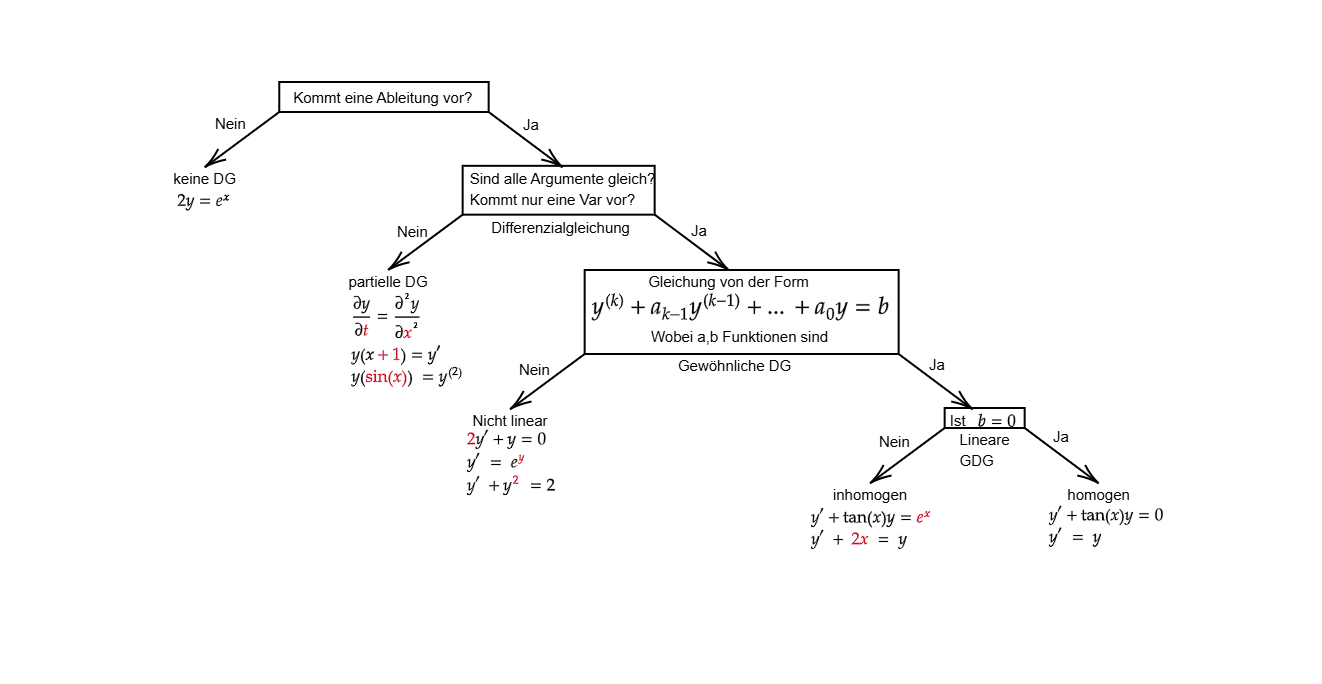
\includegraphics[scale=0.3]{build/pictures/decision_tree.png}

 


\end{multicols}
\end{document}